\chapter{COLLABORATION WITH PROXIMITY-AWARE CLUSTERING SYSTEM}
\label{chap:solare}
In this Chapter, I introduce SOLARE, a utility functions based
self-organizing network proximity-aware clustering system which can
lead to a possible performance improvement in conjunction with mobile
offloading frameworks.
%
As mentioned in Chapter~\ref{chap:scheduler} and~\ref{chap:online},
network performance such as latency and bandwidth has a significant
impact on the offloading performance, I believe that SOLARE is able to
achieve an additional performance improvement because of its ability to
organize clusters among peers which have similar network performance. 
%
However, as I will describe in this Chapter, SOLARE is the self-organizing and
managing clustering system utilizing a peer-to-peer overlay network as
an underlying substrate to place SOLARE nodes in a synthetic network
coordinate space and to propagate query messages for searching, joining,
and creating appropriate clusters.
%
Therefore, in order for mobile devices to participate directly in the SOLARE
clustering process as an overlay peer, they are required to implement basic 
functionalities of the peer-to-peer overlay networks such as
bootstrapping overlay, maintaining communication channels (i.e. near and
shortcut connections), and propagating messages from other peers, which incur an
additional overhead in terms of energy consumption and processing cost
for mobile platforms.
%
Nevertheless, there still exist ways for mobile devices to collaborate with
the network proximity-aware clustering system to improve the offloading
performance without performing the functionalities of the peer-to-peer
overlay networks. 
%
One possible collaboration of remote computation offloading with SOLARE
is a seamless service migration to another peer in a same cluster.
%
For example, in the case where a remote resource, which currently
provides computing capabilities for mobile computation offloading,
becomes not available due to resource crashes or network problem, the
offloading service should be migrated to another remote resource.
%
If the mobile device keeps a list of remote resources which guarantee
similar network performance in terms of latency or bandwidth (i.e.
remote resources having the same cluster membership) and seamlessly
hopping into another remote resource in the same cluster, the offloading
service is able to continue without any service disconnection or restart.
%
Thus, with the assist from SOLARE, mobile offloading frameworks do not
have to repeat the service discovery process to find another remote
resource which has the best network performance and the offloading
service can resume seamlessly.
%
\section{Motivation of SOLARE}
\label{solare:motivation}
In recent years, the structures of large-scale network have been
extended from client-server architectures for traditional web services
to the distributed systems such as Peer-to-Peer (P2P) networks and
Distributed Hash Tables (DHTs)~\cite{chord, can, tapestry}.
%
Particularly, distributed systems have been increasingly applied to
applications including online gaming, content distribution networks, and
storage systems.
%
One of the key challenges posed by these systems is locating or
connecting a subset of nodes that satisfy user-demands with respect to
network proximity.
%
In distributed online gaming services, for example, players seek to
organize cluster so that those in the same cluster can experience low
latency to each other and enjoy the game without delay perceived by
users.
%
In addition, the supply of powerful commodity computers and the
availability of high speed Internet have enabled grid computing
environments capabilities.
%
In such environments, latency-sensitive applications such as parallel
processing tasks and workflows benefit from proximity among workers, and
the ability to discover resources which satisfy job demands and are
bound by pair-wise latency constraints is important.
%
For such reasons, the inherent support for large-scale systems to
self-organize into clusters that guarantee a certain degree of network
proximity allows middleware and applications to seamlessly discover
resources that are close in a network latency sense.
%
With the approach described in this Chapter, proximity-aware queries can
be efficiently performed through scalable P2P queries within the
self-organized cluster(s) that a node belongs to.\\
%
SOLARE is a peer-to-peer, utility function based self-managing system
that self-organizes clusters in a proximity-aware structured overlay
topology.
%
To do this, I rely on a structured P2P network as underlying global
overlay network and a self-organizing, decentralized network coordinate
system.
%
As reviewed in the next section, there have been a number of related
approaches whereby nodes are clustered based on certain criteria, but to
the best of our knowledge, this work proposes the first implementation
which applies utility functions and network coordinates for the
clustering process.
%
The main idea of SOLARE is that each node searches and joins the highest
utility valued cluster.
%
On the other hand, if there is no cluster whose utility is greater than
the user-defined threshold, the node creates a new cluster declaring its
own coordinate as the virtual center of cluster.
%
Furthermore, a node periodically monitors the status of the cluster that
it is currently involved in so that the node migrates to another cluster
whenever the utility is dropped below a threshold.
%
In this system, migrating clusters means changing the cluster membership
rather than physically moving from one cluster to another cluster.
%
In order to calculate the utility of clusters, I select the distance to
the virtual center of the cluster and the size of the cluster (i.e. the
number of current cluster members) as utility properties.
%
All participants are located in a 2-dimensional space such that each
node has the ability to calculate the Euclidean distance to any points
of 2-dimensional space or other nodes using a Vivaldi network coordinate
system~\cite{vivaldi}.
%
It is important to note that SOLARE is independent of the network
coordinate system.
%
In fact, even though I adopt the Vivaldi network coordinate system,
other related approaches such as GNP~\cite{gnp} and PIC~\cite{pic} can be used for the core of
network latency prediction of SOLARE as well.
%
While this Chapter focuses on latency-based network coordinates,
approaches that consider a bandwidth-based coordinate systems, such as
Sequoia~\cite{ramasu, treeness} can be also considered.
%

\section{Related Work}
\label{solare:related}
\subsection{Clustering approaches on distributed systems}
\label{solare:clustering}
Similar studies to this work have been done in order to offer
proximity-based routing protocols.
%
In~\cite{locality} , the Plethora routing core employs a two-level overlay architecture
with global overlay and local overlays.
%
In particular, local overlays rely on the organization of the Internet
as a collection of Autonomous Systems (ASs) so that they serve as caches
to provide data locality.
%
IP-based clustering for P2P networks has no need for active measurement
of latencies, minimizing system maintenance cost~\cite{ipclustering}.
%
Instead, the authors provide a simple method for the construction of
clusters based on static, readily available information (i.e. IP
address) proving the correlation among common UP prefix length of
communication nodes and latency.
%
The above approaches, however, use only static information without any
measurements, which makes it difficult to handle dynamic network
changes.
%
Cantin et al.~\cite{cantin} adopt the Quality Threshold (QT) algorithm to propose a
self-organized clustering scheme which is built on an existing Internet
coordinate system.
%
Also, they present two variants of distributed clustering algorithm: one
aims at reduction of the clustering construction time, the other tries
to minimize the overhead of the clustering process.
%
Nevertheless, each node needs to perform the computation for QT
algorithm as well as calculating the distance between its first- and
second-order neighbors, introducing additional overheads.
%
The novelty which distinguished this work from the aforementioned
approaches is that this work is a fully decentralized and autonomous
approach, not relying upon any central units such as servers, super
peers, cluster heads or landmarks but utilizing utility functions.\\
%
Clustering techniques have been also adopted in other domains such as
network modeling and performance evaluation.
%
In~\cite{filesharing}, the authors show that both geographical and interest-based
clustering properties inherently exist and can be leveraged to improve
the search mechanisms in file sharing systems using P2P networks.
%
Bu et al.~\cite{bu} provide the Internet topology generator using the cluster
coefficient.
%
Also, wireless sensor networks achieve prolonging the lifespan and
reducing the overhead via cluster-based protocols~\cite{clusterrouting,
energyintra, cao}.
%

\subsection{Utility functions in autonomous systems}
\label{solare:utility}
Utility functions provide a natural and advantageous framework for
achieving self-optimization in autonomic computing~\cite{utilityself}.
%
In fact, applying utility functions to autonomic systems has been done
in various studies.
%
In~\cite{william, unity}, the authors have proposed utility-based resource allocation system
consisting of a number of logically separated application environments
each having an independent utility function.
%
Along with application environments, a global resource arbiter performs
the allocation of resources optimizing the summation of utility
functions from application environments.
%
Similar work has been considered in~\cite{directed}.
%
In this work, however, utility is described with respect to low-level
resources such as CPU, disk, and memory instead of system-level
attributes.
%
In~\cite{cooling}, the authors propose an energy efficient cooling system for data
centers applying utility functions.
%
It formulates simple utility functions that describe a trade-off between
energy and temperature and shows how to optimize a setting of control
parameters, fan speeds and on/off state of air conditioners, using
utility functions.
%
Grandis et al.~\cite{grandis} present the fundamental steps of non-analytic approach on
leveraging utility functions at the application level.
%
Also, they apply their approach to two different case studies, FTP
download and log explosion.
%

\begin{figure}
\centering
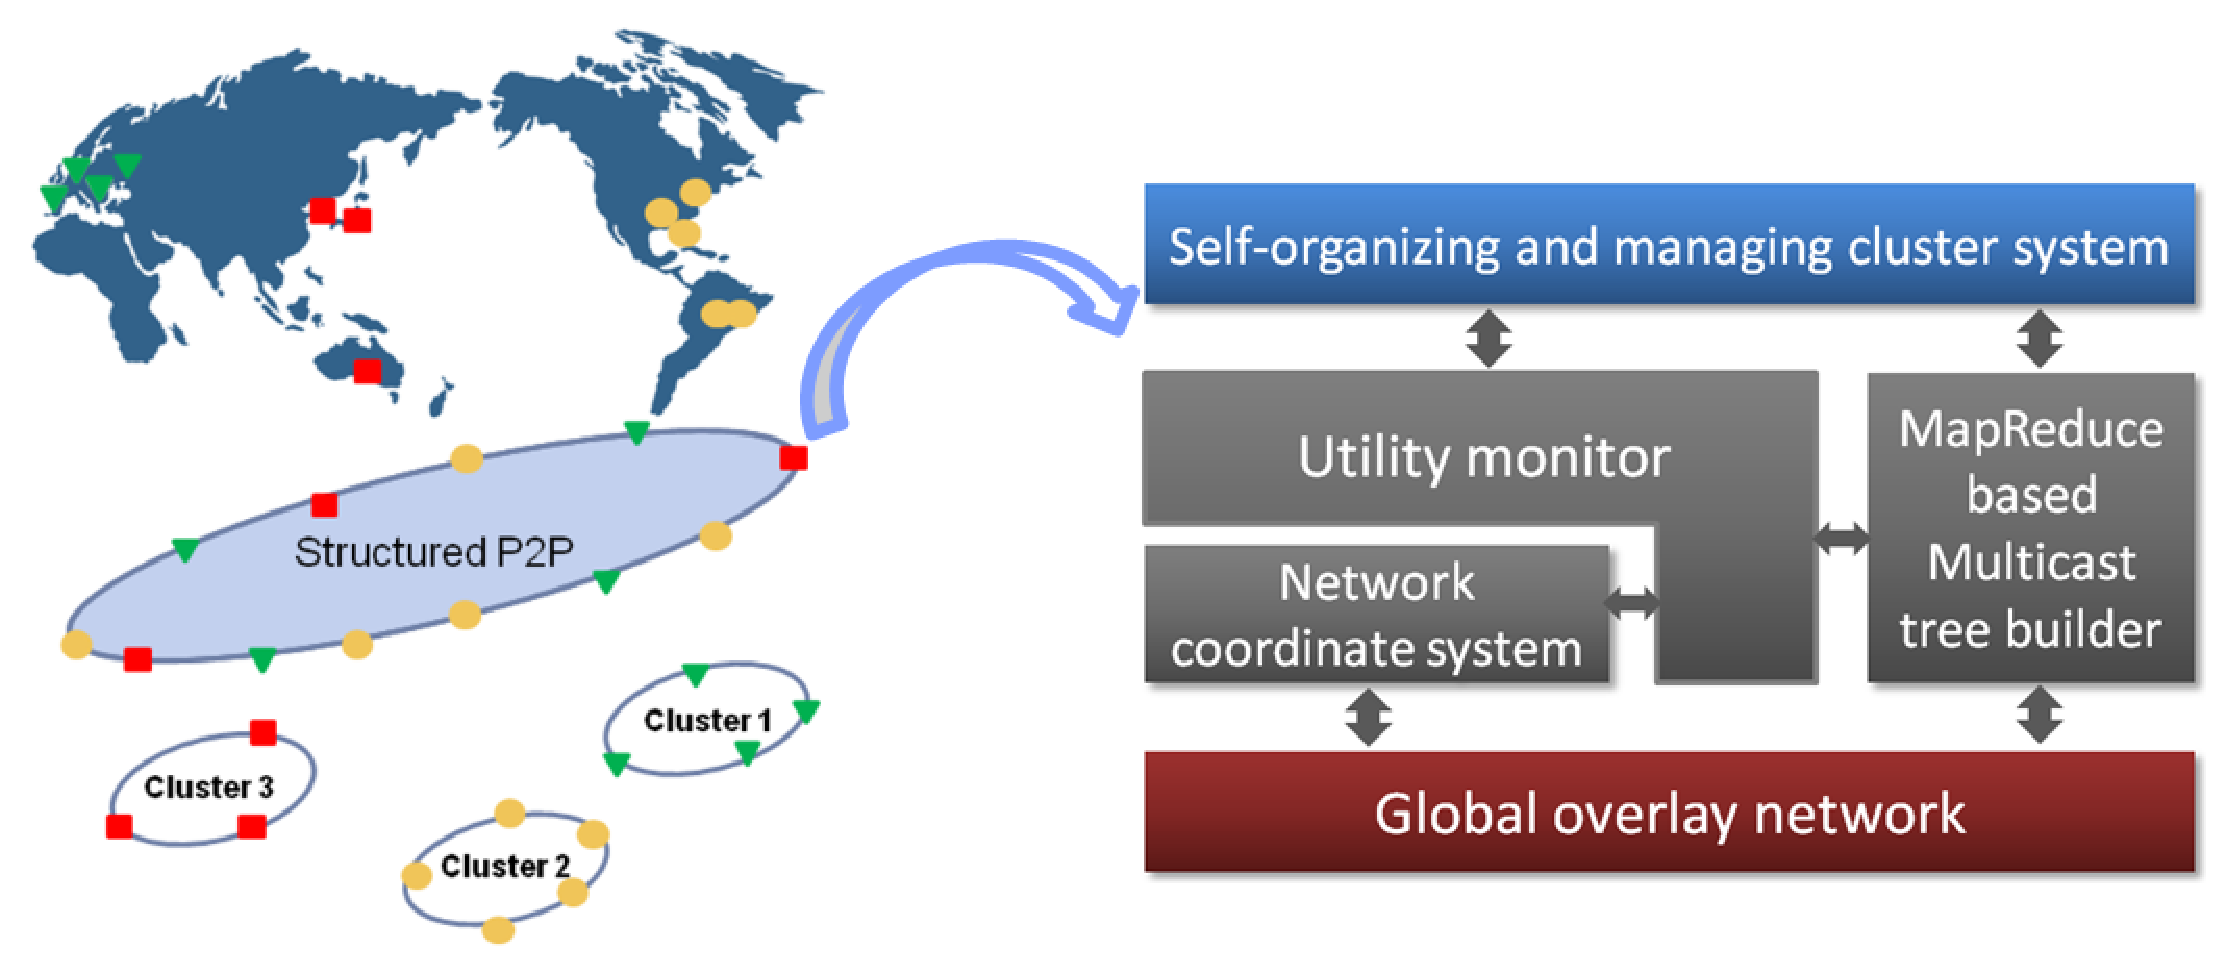
\epsfig{file=figs/solare_structure.eps, width=5.5in}
\caption{Self-organizing latency-aware resource ensemble}
\label{fig:solare}
\end{figure}
%

\section{System Model and Architecture}
\label{solare:architecture}
The main goal in SOLARE is to construct utility functions-based,
self-organizing and self-managing cluster systems such that nodes join
highest ranked cluster with respect to its own preference expressed by a
utility function.
%
The system assumes a global, large-scale structured P2P overlay, from
which virtual clusters are self-organized as sub-overlays based on the
SOLARE algorithm.\\
%
Figure~\ref{fig:solare} illustrates the base concept of the SOLARE
system.
%
In this figure, three small-scale clusters self-organize as virtual
sub-overlays (triangle, circle, square) of the main global overlay based
on their network coordinates and utility functions.
%
Furthermore, each node monitors the cluster that it is currently
involved in, so if its utility value drops below a threshold due to
dynamic changes in network conditions, it migrates to another cluster to
improve cluster utility.
%
Consider, for example, nodes that are geographically distributed and
connected to a large-scale overlay with millions of nodes.
%
Assume a node wishes to connect to 100 nodes or more which are within 50
milliseconds of latency (i.e. round trip time).
%
This node specifies its desirable cluster characteristics in terms of a
utility function, and takes part in SOLARE on top of global overlay
network, requesting information from existing clusters through a
bounded-multicast query mechanism which discovers which nodes belong to
clusters that would maximize the node's utility.
%
Finally, the node makes a decision on the best-suitable cluster based on
its requirements.
%
These steps involve the modules shown in Figure~\ref{fig:solare}
(right).
%
In this section, I describe the main constituents of SOLARE.
%

\subsection{Structured P2P network as global overlay}
\label{solare:global}
The global overlay network provides an underlying substrate to place
nodes in a network coordinate space and to propagate query messages.
%
As soon as nodes join the global overlay network, they calculate their
positions and send a query message for cluster information.
%
I choose Symphony~\cite{symphony}, a 1-dimensional Kleinberg small-world network as
underlying global overlay network, and build upon the implementation of
Brunet~\cite{brunet}, a general P2P software framework.
%
Symphony organizes nodes in a ring topology in which each node has a
constant number of near connections and \textit{log(N)} number of
shortcut connections, where \textit{N} is the number of nodes in the
network.

\subsection{Query propagation system}
\label{solare:query}
One of the essential features of a self-organizing cluster system is how
nodes locate a candidate set of clusters in an efficient way, without
missing high-quality clusters to join in terms of the user demand.
%
With the purpose of improving the cluster searching quality with
scalable query mechanism, I employ Map and Reduce functions on a
self-organizing multicast tree~\cite{lee}.
%
This approach is based on a multicast tree builder consisting of two
parts: Map and Reduce functions which process the propagation of query
and merge the results, and a multicast tree builder that is the
recursive algorithm to build a multicast tree.
%
MapReduce is a software framework associated with information processing
on large data sets~\cite{mapreduce}.
%
The Map function works on a set of data to generate intermediate value
while the Reduce function merges all intermediate value associated with
the identical intermediate key.
%
In conjunction with Map and Reduce functions, the multicast tree
builder assists in propagating a message in a scalable manner (with
\textit{log(N)} depth) by building a multicast tree using structured
shortcut and near connections~\cite{deetoo}.
%
This approach can be applied recursively to
sub-overlays~\cite{bootstrap} such that the
same mechanism used across the overlay to discover candidate clusters to
be joined, can also be used at the application layer to discover nodes
that satisfy requirements within a proximity-aware cluster.\\
%
\begin{figure}
\centering
\subfigure[Symphony topology] {
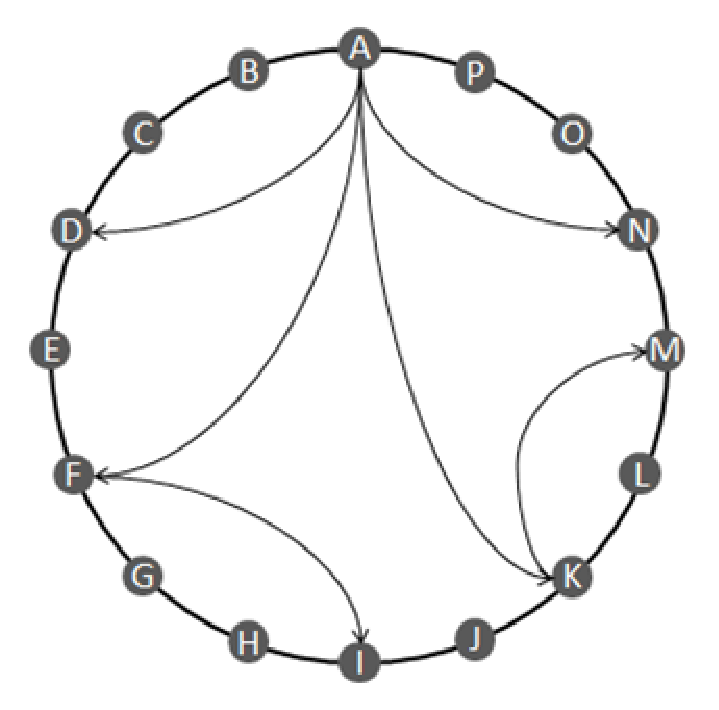
\includegraphics[width=2.3in]{figs/symphony.eps}
\label{fig:symphony}
}
\subfigure[Multicast tree] {
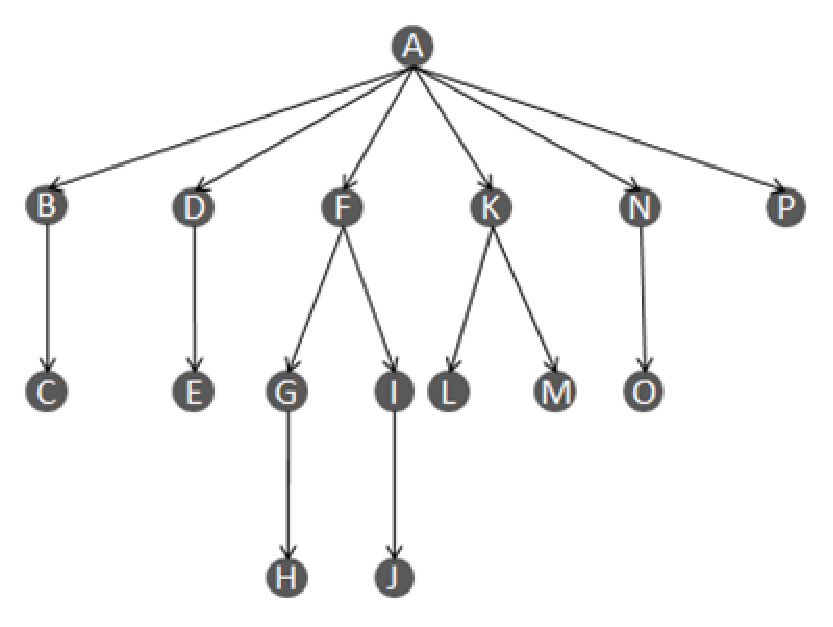
\includegraphics[width=2.3in]{figs/multicast_tree.eps}
\label{fig:multi}
}
\caption{Map and Reduce functions based multicast tree builder}
\label{fig:treebuild}
\end{figure}
%
Figure~\ref{fig:treebuild} shows how Map and Reduce functions based
multicast tree builder creates the multicast tree and propagates a query
on top of symphony.
%
Assuming that node A is an origin node which sends a message over the
entire network (or alternatively a bounded region of the network, in
this example the bounds are A and P).
%
Node A sends a message to nodes B, D, F ,K, N and P (which are referred
as node A's child nodes) through its near connections and short
connections by setting sub-multicast range as [B,D), [D,F), [F,K),
[K,N), [N,P) and [P,A-1), respectively.
%
Nodes which receive the message send the message to their neighbors
within sub-multicast range.
%
Differently stated, node B has the responsibility of building the
multicast tree in range [B,D).
%
In a such way, nodes multicast the message until there is no connection
and the multicast tree is built as shown in Figure~\ref{fig:multi}.
%
Each node in the tree computes a Map function, and results are
back-propagated through the tree, with each node computing a Reduce
function on the values they receive from its children.
%
The strength of Map and Reduce functions based multicast tree builder
lies in the ability to parallelize the Map and Reduce functions,
providing the ability to select a subset of results based on utility
functions, thereby bounding the bandwidth used in such queries.
%
With a Reduce function that bounds the number of results returned by a
node by a constant, the average per-node bandwidth consumed by a query
is constant~\cite{deetoo, lee}.
%

\subsection{Network coordinate system}
\label{solare:coordinate}
A network coordinate system places nodes in some synthetic network
coordinate space such that each node can predict the latency to other
nodes.
%
One example is Vivaldi, which achieves this by modeling a spring
system~\cite{vivaldi}.
%
Due to the triangle inequality of the network coordinate space, the Vivaldi
network coordinate system attempts to minimize the error between the
predicted distance and actual latency instead of exploiting accurate
coordinates.
%
Each node involved in the Vivaldi network coordinate system measures the RTT
(Round Trip Time) to its neighbor \textit{n$_{i}$} whose coordinate is
\textit{x$_{i}$} and computes the error \textit{e} between measured RTT
and Euclidean distance of its coordinate and \textit{x$_{i}$}.
%
Finally, it updates its new coordinate as follows:
%
\begin{equation}
	\textit{Coordinate$_{new}$} = \textit{Coordinate$_{previous}$} +
\textit{$\delta$} \times \textit{e} \times \textit{D} 
\label{equ:coordinate}
\end{equation}
%
where $\delta$ is the timestep which quantifies the size of step toward
new coordinate and \textit{D} is the direction to new coordinate.
%
An adaptive value of $\delta$ provides the control on the fraction of
the step so that each node converges towards approximately accurate
position quickly and precisely.
%
The Vivaldi system has been implemented on top of Brunet and is used as
a basis for the experiments in this work.
%
As soon as each node joins the global overlay, it runs the Vivaldi
network coordinate system to obtain 2-dimensional coordinates so as to
predict the latency to the candidate clusters as well as the neighbors.
%

\section{SOLARE Modules and Algorithms}
\label{solare:modules}
\subsection{Utility functions}
\label{solare:utility}
A self-organizing and self-managing system needs to serve diverse
requests from a number of users who have different expectations on
service quality.
%
The challenge of this task is not only to approximately satisfy the
demands from all the users but also to maximize the utilization of
entire system.
%
In this work, I make use of utility functions as a practical scheme of
achieving self-organizing and self-managing cluster system in which each
node describes its own preference on joining a cluster, and makes the
best decision given a set of clusters.
%
To apply utility functions to this system, first of all, I identify two
attributes that nodes attempt to optimize.\\
%
\textbf{Distance to the cluster (\textit{D$_{i}$}).} means the Euclidean
distance between the coordinate of node and a virtual center of a
particular cluster, \textit{i}.\\
%
\textbf{Size of cluster (\textit{S$_{i}$}).} is the size of a cluster,
that is  the number of cluster members which involve in a particular
cluster, \textit{i}.\\
%
Next, I establish two utility functions, \textit{U$_{distance}$} and
\textit{U$_{size}$}, each expressing the preference on above two
attributes.
%
\begin{figure}
\centering
\subfigure[Utility for Distance(\textit{D$_{max}$} = 100)] {
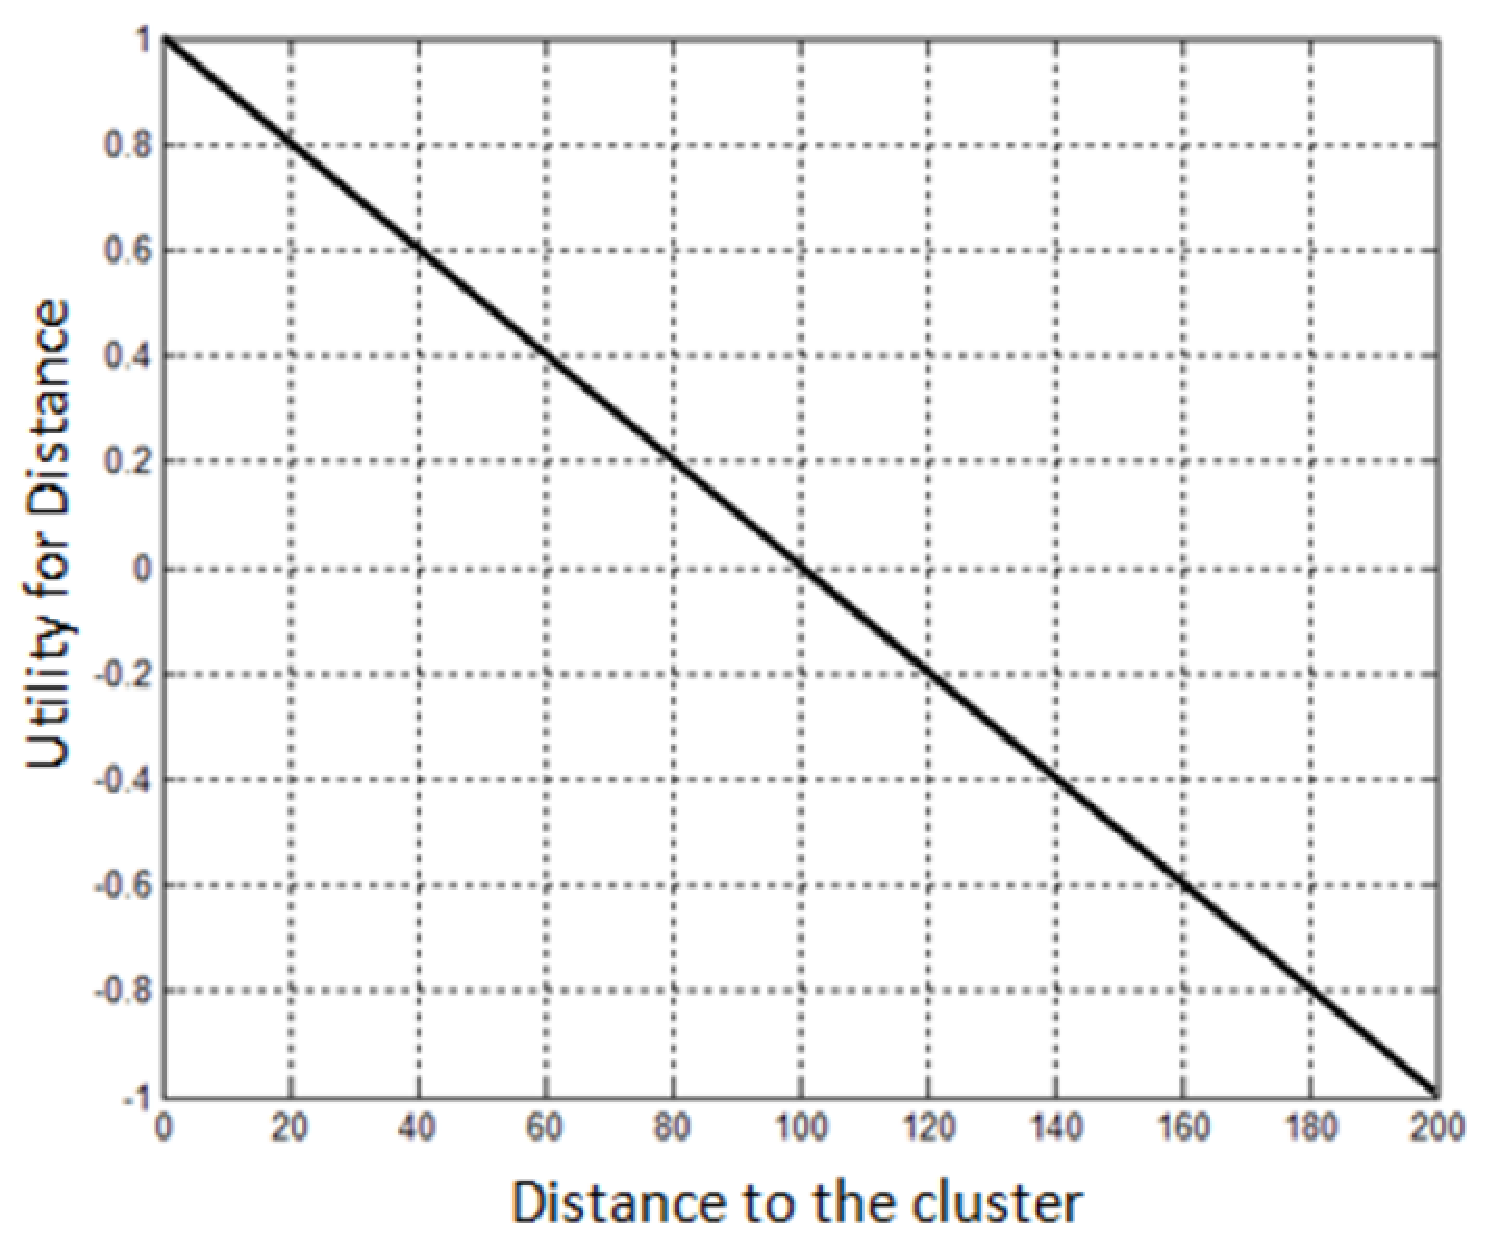
\includegraphics[width=2.7in]{figs/utility_distance.eps}
\label{fig:udistance}
}
\subfigure[Utility for Size(\textit{S$_{min}$} = 100)] {
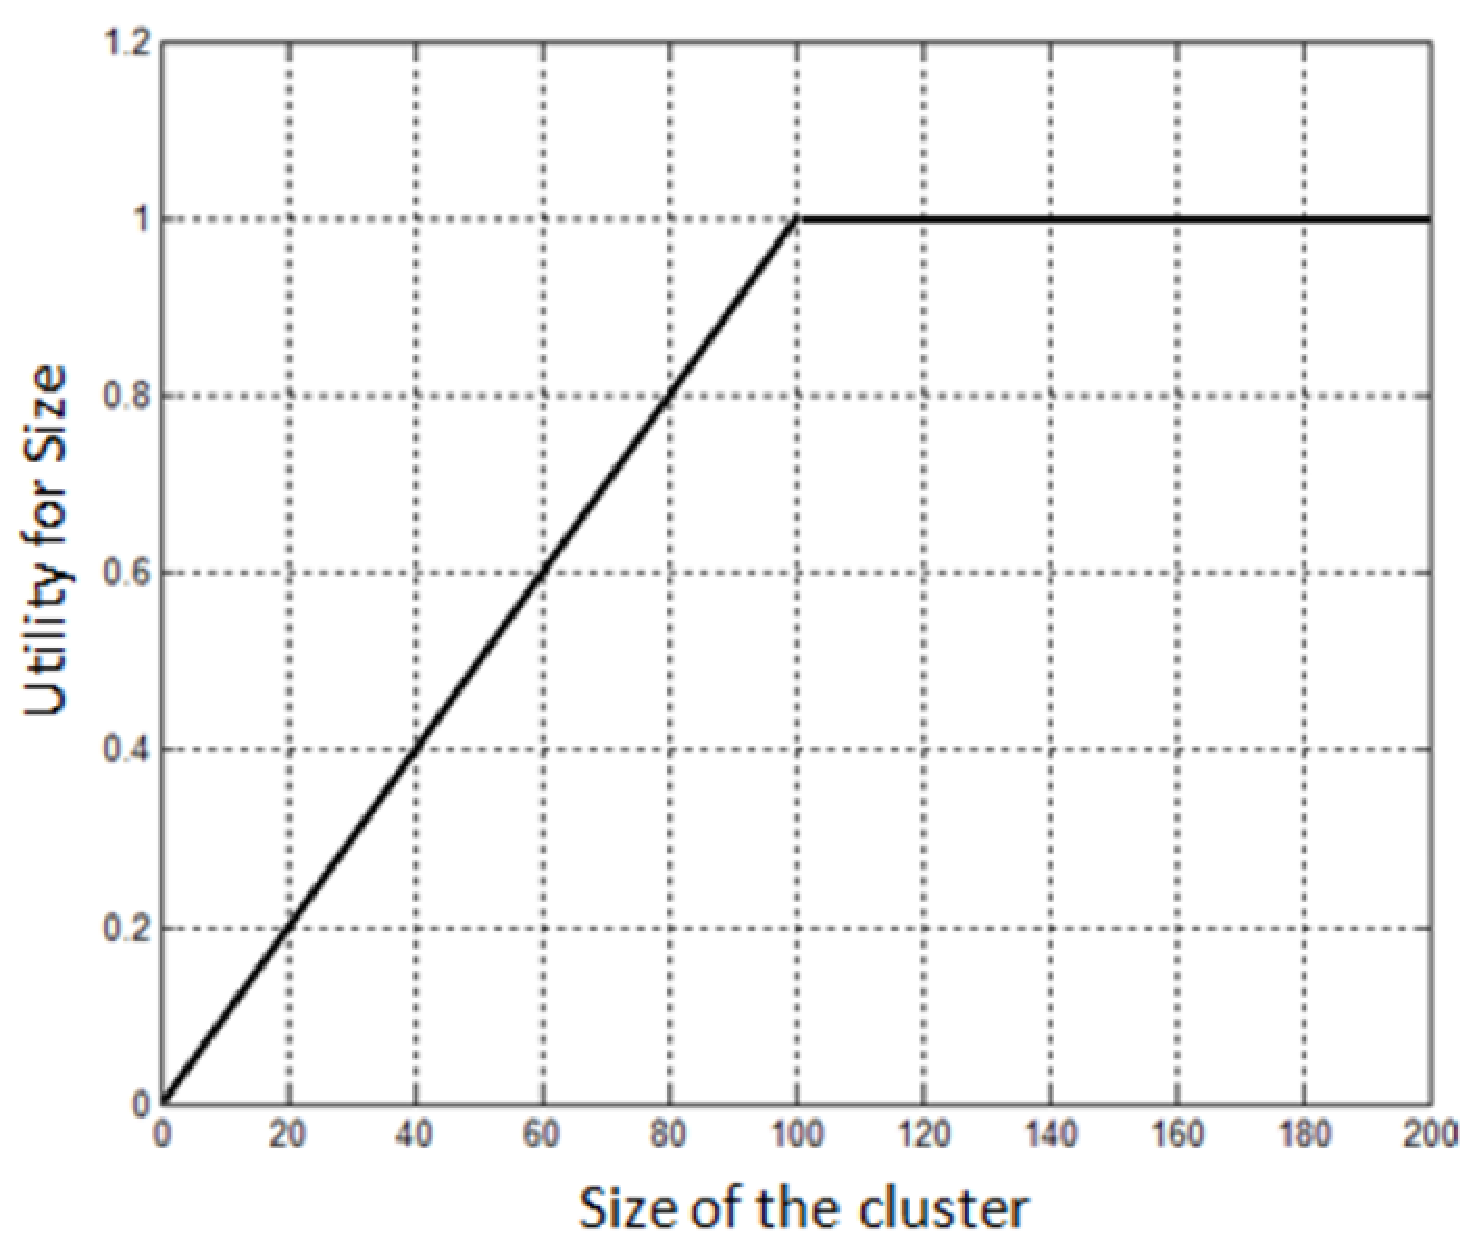
\includegraphics[width=2.7in]{figs/utility_size.eps}
\label{fig:usize}
}
\caption{Example for utility functions for cluster distance and size}
\label{fig:utility}
\end{figure}
%
Figure~\ref{fig:utility} illustrates utility functions \textit{U$_{distance}$} and
\textit{U$_{size}$} that I set in this system.
%
Note that I have two key parameters to configure: maximum tolerance for
distance to the virtual cluster center (\textit{D$_{max}$}) and minimum
preference for cluster size (\textit{S$_{min}$}).
%
The former is the maximum distance to the cluster which has positive
utility value, while the latter means the minimum size of the cluster
which has maximum utility, 1, regardless of the size of the cluster.
%
Users can define their own utility functions by differently setting
these two parameters.
%
Finally, after adding the coefficients for each utility function, I
merge two utility functions into total utility function as
Equation~\eqref{equ:utility} in which each node computes total utility
value for a cluster.
%
\begin{equation}
	\textit{U$_{total}$} = \textit{$\alpha$$_{size}$} \times
\textit{U$_{size}$} + \textit{$\alpha$$_{distance}$} \times
\textit{U$_{distance}$} 
\label{equ:utility}
\end{equation}
%
where \textit{$\alpha$$_{size}$} and \textit{$\alpha$$_{distance}$} are
coefficients for \textit{U$_{size}$} and \textit{U$_{distance}$},
respectively, such that the sum of two values is 1.
%
Similar to \textit{D$_{max}$} and \textit{S$_{min}$}, coefficients for
size and distance are user-definable parameters so that each user
presents the priority among the attributes.
%
\begin{figure}
\centering
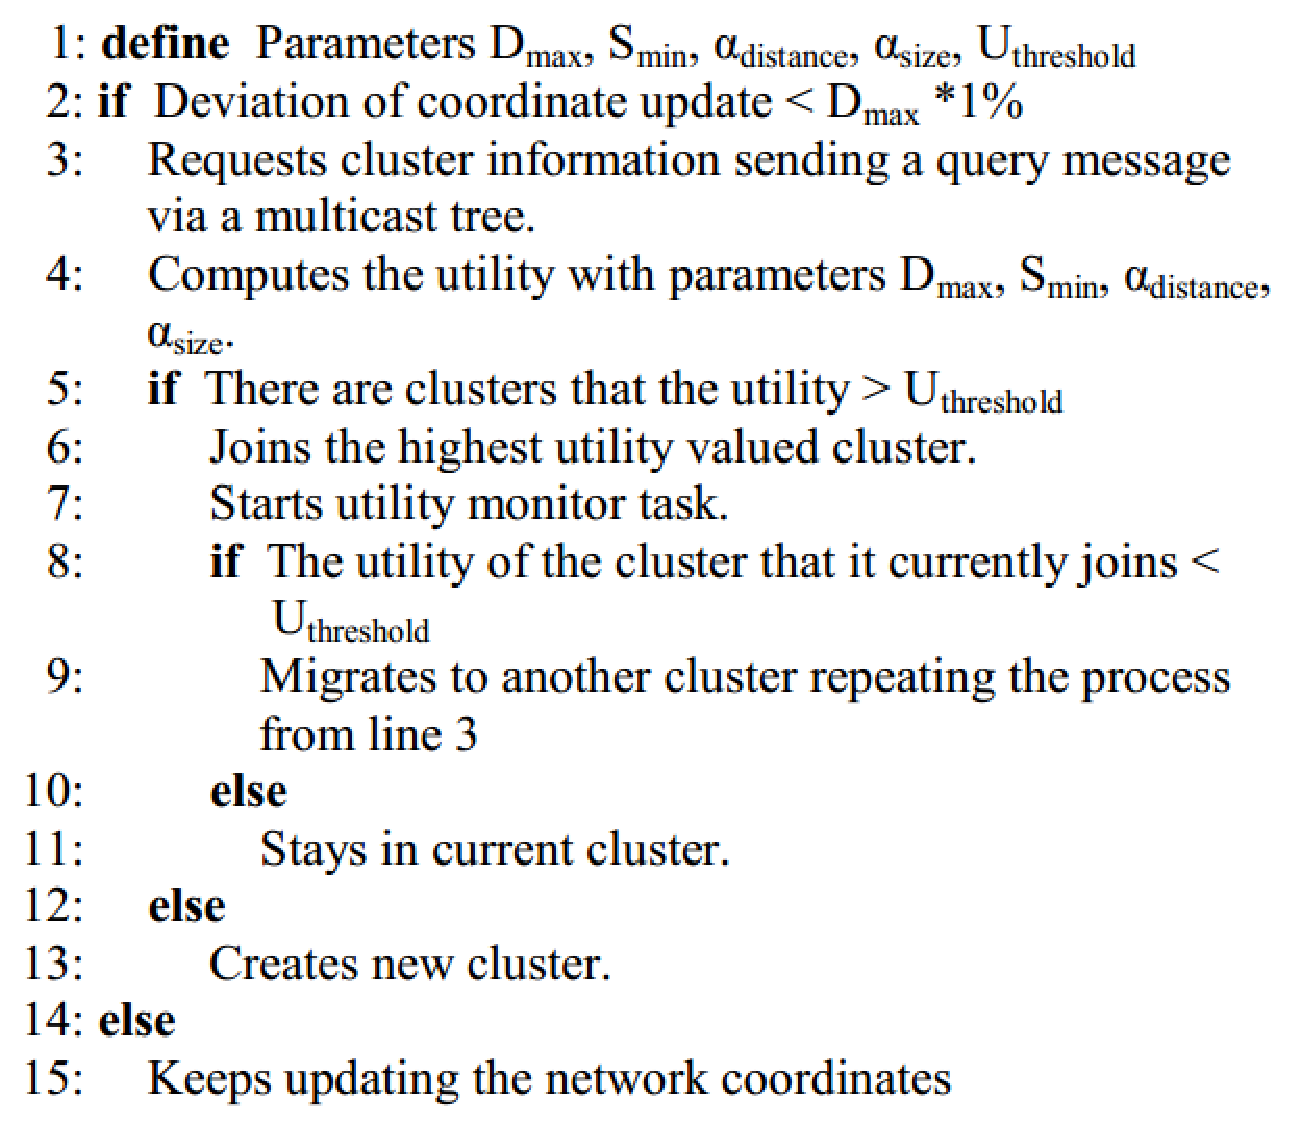
\epsfig{file=figs/solare_algorithm.eps, width=4.3in}
\caption{Pseudo-code for self-organizing and managing clustering system}
\label{fig:solare_algorithm}
\end{figure}
%

\subsection{Self-organizing and managing cluster process}
\label{solare:clusterprocess}
As described in previous section, utility functions represent user
preference on selecting a cluster to join.
%
In this section, I describe how nodes can self-organize the cluster
architecture using utility functions.
%
The main idea of this clustering algorithm is that each node searches
and joins the highest utility valued cluster.
%
On the other hand, if there is no cluster whose utility is greater than
the user defined threshold, nodes create new cluster declaring its own
coordinate as the virtual center of cluster.
%
Furthermore, a node periodically monitors the status of cluster that it
is currently involved in order to migrate to another cluster whenever
the utility is dropped below the threshold.
%
The clustering process is presented in Figure~\ref{fig:solare_algorithm} 
and described in detail as follows.\\
%
Upon joining the global network, a node computes its coordinates in
2-dimensional Euclidean space using Vivaldi network coordinate system.
%
In order to avoid too frequent cluster migrations on the way toward the
accurate position, the cluster process starts after the deviation of
coordinate update becomes relatively small.
%
As soon as node initiates the clustering process, it sends a request
message including its coordinates to find the highest utility valued one
of existing clusters through the multicast tree constructed by Map and
Reduce functions based multicast tree builder.
%
As the response for the request message, all the nodes calculate the
utility of its cluster using the coordinate of the query origin node
with the Map function and compare the utility of its cluster to the
utilities from its child nodes using the Reduce function.
%
Then, nodes send only the information of the highest utility valued
cluster to their parent node of the multicast tree.
%
As a result, the query origin node receives only one response from a
child node, and it can find the highest utility valued cluster with a
lightweight comparison.
%
It is worth noting that Map and Reduce functions at the response phase
help in reducing the number and the size of response messages.
%
After joining the highest utility valued cluster, the node informs
cluster members of its intent to join by multicasting a join message.
%
By counting this type of message, cluster members keep the size of
cluster up to date; they can also periodically query the cluster for
membership count using a Map and Reduce functions multicast query within
the cluster sub-overlay.
%
If utility values of all the existing clusters do not satisfy the demand
of the node (which means that utility values are less than the
user-defined threshold), the node creates a new cluster.\\
%
Creating a new cluster is straightforward.
%
A node generates a random clusterID ranging from 0 to 2$^{160}$-1 which is
identical to the node address space of Symphony.
%
Also, the node declares its current coordinates as the virtual center of
cluster.
%
With doing this, the node can subsequently reply to cluster requests
from other nodes.
%
After first joining the cluster, the node starts a utility monitoring
task.
%
Network status has the possibility to be changed due to the churn and
dynamic changes in traffic in the physical network.
%
Such changes in the network result in the fluctuation of the utility
value and nodes can take the potential advantage from the ability to
migrate from the current cluster to another cluster.
%
The self-managing cluster system needs to deal with this problem.
%
The utility arbiter checks whether utility value is dropped below the
threshold or not.
%
To do this, nodes  periodically calculate the distance to the virtual
center of cluster and count the number of cluster members.
%
If the utility value is dropped below the threshold, nodes repeat above
cluster searching, joining or creating process.\\
%
The main contribution of this work is that the clustering algorithm has
a fully decentralized feature which does not rely upon any central units
such as servers, super peers, cluster heads or landmarks; hence it is
robust against the single point of failure.
%
Because each node holds the information of its own cluster locally, it
is unlikely that node failures or leave affects the performance of the
whole system.
%
Also, the destruction of cluster which does not have any cluster members
at all is done without additional process.
%
The departure of last cluster member means that the cluster does not
exist in the network.
%

\section{Performance Evaluation}
\label{solare:evaluation}
In this section, I present results from simulation based analysis for
SOLARE.
%
In this evaluation, I use Brunet in event-driven simulation
mode~\cite{david} and
configure simulated latencies using King dataset~\cite{king} with 1740 nodes.
%
Brunet simulator uses simulated virtual time based upon an event-driven
scheduler instead of real time.
%
While existing simulators such as p2psim~\cite{p2psim}, NS2~\cite{ns2},
and netmodeler~\cite{netmodeler} are
algorithm-oriented simulators which aim to evaluate algorithm
validation, Brunet simulator has the ability to simulate the deployed
system stack as well as algorithm using a specialized transport layer to
avoid the overhead of using TCP or UDP on the host system.
%
The specialized transport uses datagrams to pass messages between nodes,
thus from an individual node's perspective, it is very similar to a UDP
transport and can simulate both latency and packet dropping.
%
\begin{figure}
\centering
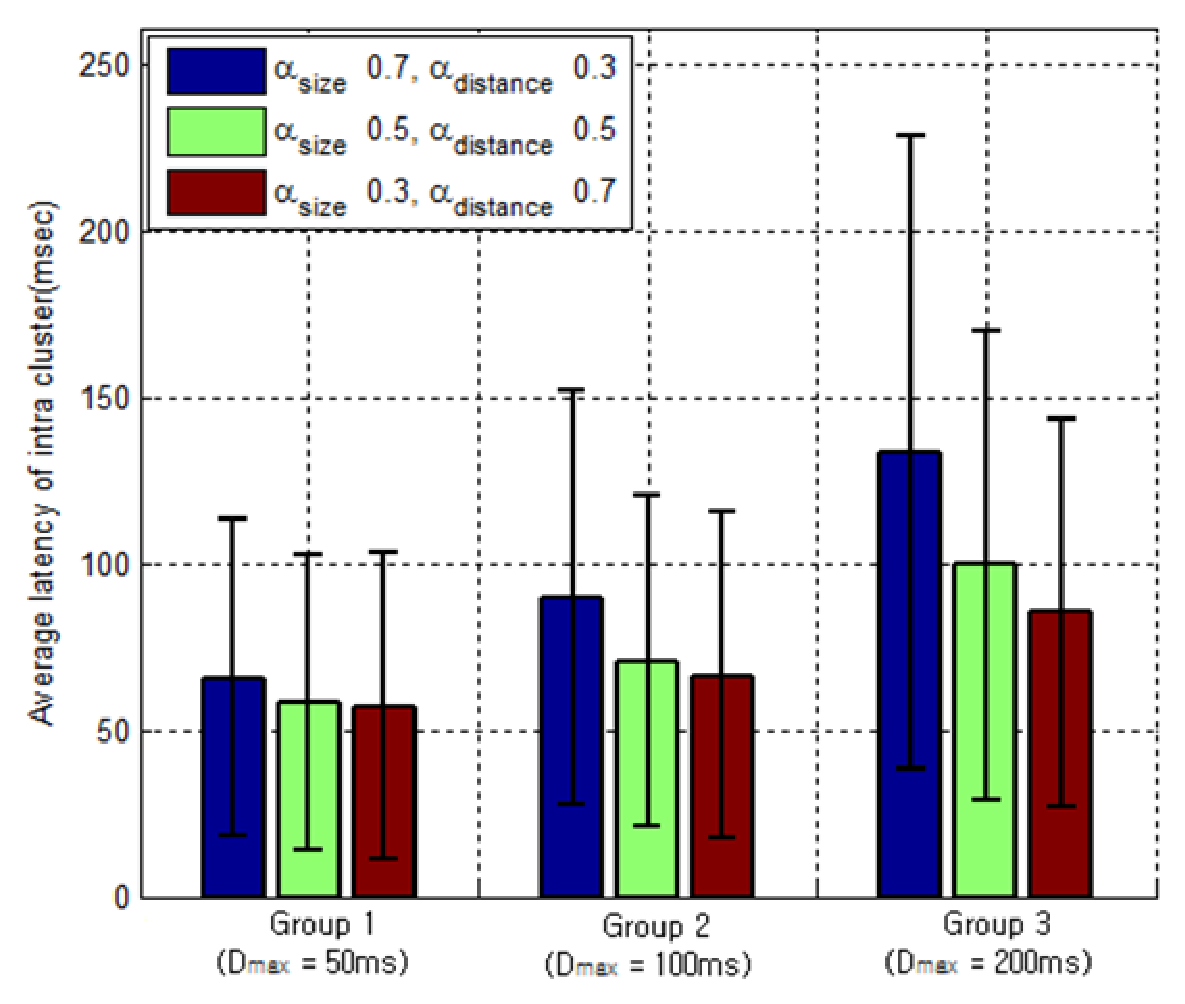
\epsfig{file=figs/latency_s50.eps, width=4.0in}
\caption{Average latency of intra-cluster with \textit{S$_{min}$} = 50}
\label{fig:latency50}
\end{figure}
%
\begin{figure}
\centering
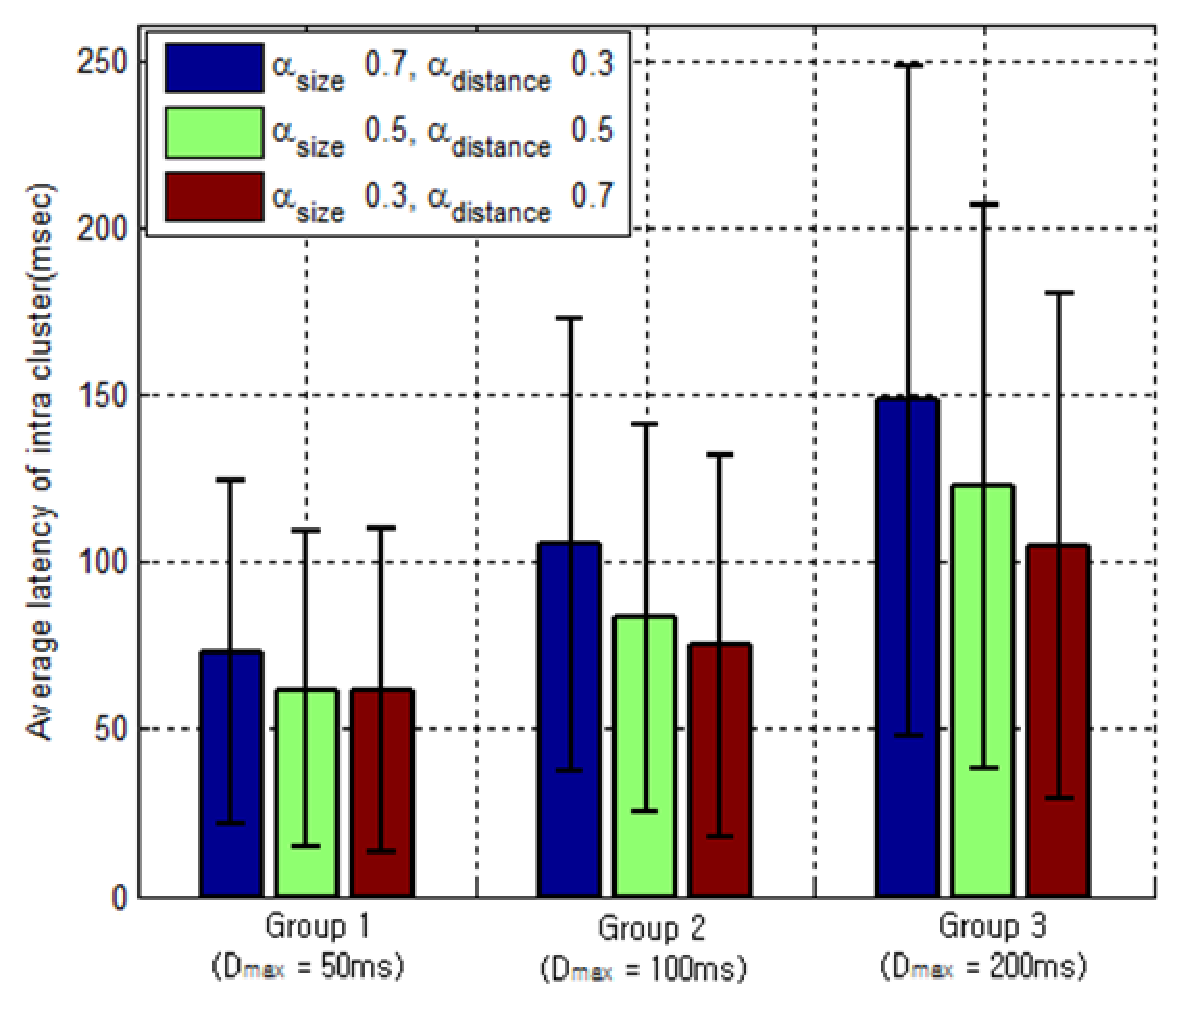
\epsfig{file=figs/latency_s100.eps, width=4.0in}
\caption{Average latency of intra-cluster with \textit{S$_{min}$} = 100}
\label{fig:latency100}
\end{figure}
%
\begin{figure}
\centering
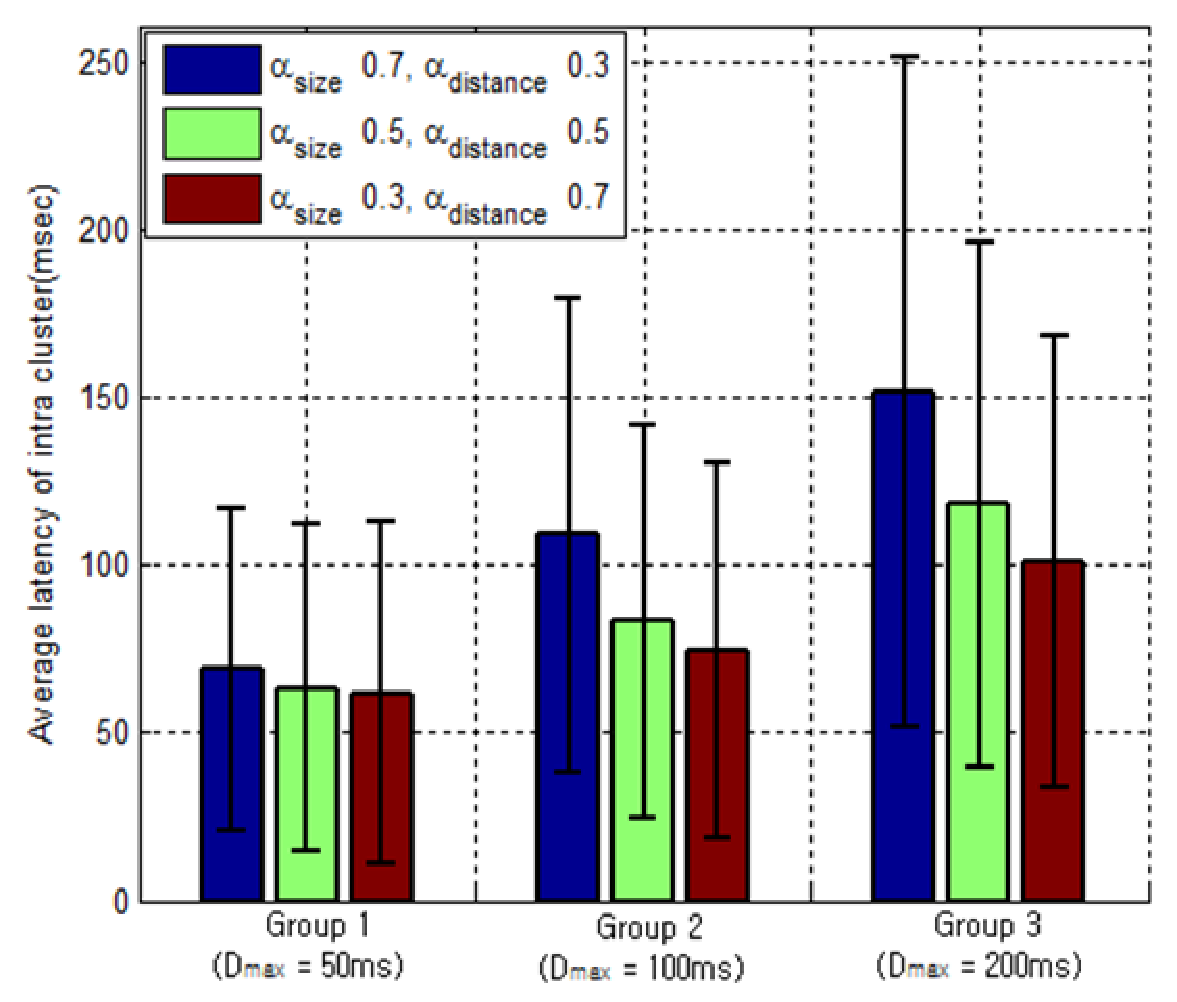
\epsfig{file=figs/latency_s200.eps, width=4.0in}
\caption{Average latency of intra-cluster with \textit{S$_{min}$} = 200}
\label{fig:latency200}
\end{figure}
%

\subsection{Inter-cluster latencies}
\label{solare:interlatency}
Since \textit{D$_{max}$} is the maximum distance to the virtual cluster
center that a node expects when it searches a cluster to join, I can
refer \textit{D$_{max}$} as the radius of cluster.
%
Therefore, upon joining a particular cluster, nodes are able to expect
at most 2$\times$\textit{D$_{max}$} of the latency between cluster
members.
%
To evaluate the performance of this clustering algorithm, I measure
intra-cluster latencies -- the latency between cluster members in the
same cluster.
%
I set \textit{D$_{max}$} to 50ms, 100ms, and 200ms, and
\textit{S$_{min}$} to 50, 100, and 200, respectively.
%
Also, \textit{$\alpha$$_{distance}$} is varied with 0.3, 0.5, and 0.7 (i.e.
\textit{$\alpha$$_{size}$} is 0.7, 0.5, and 0.3).
%
Figure~\ref{fig:latency50},~\ref{fig:latency100},
and~\ref{fig:latency200} show the average and standard deviation of
intra-cluster latency with various parameters setup.
%
First of all, I observe that all the combinations of the parameters
satisfy 2$\times$\textit{D$_{max}$} in terms of the average latency of
intra-cluster.
%
Specially, even in all cases that \textit{D$_{max}$} is 50ms, the
average latency is less than 2$\times$\textit{D$_{max}$}, 100ms.
%
From this result, I note that even though nodes only measure the
distance to the virtual center of cluster, it does not prevent nodes
from getting neighbors who are mostly within \textit{D$_{max}$}.\\
%
Second, by comparing three bars which have different colors in each
group, I observe that the larger coefficient for distance,
$\alpha$$_{distance}$ is, the smaller average intra-cluster latency is.
%
In the case that \textit{D$_{max}$} is 50ms in
Figure~\ref{fig:latency50}, the average
intra-cluster latency with $\alpha$$_{distance}$ of 0.7 is reduced by
11\% and 2\% compared with $\alpha$$_{distance}$ of 0.3 and 0.5,
respectively.
%
Such this difference becomes much clearer as \textit{D$_{max}$}
increases showing 35.9\% and 14.4\% of decrease compared the case of
$\alpha$$_{distance}$ of 0.7 with the cases of 0.3 and 0.5 and
\textit{D$_{max}$} of 200ms.
%
The standard deviation when $\alpha$$_{distance}$ is set to 0.7 is also
decreased by 38.7\% and 17.2\% compared to $\alpha$$_{distance}$ of 0.3
and 0.5 in the Group1 of Figure~\ref{fig:latency50}.
%
Furthermore, I observe that the minimum preference for cluster size,
\textit{S$_{min}$} does not affect the average intra-cluster latency by
observing the same pattern of average latency regardless of
\textit{S$_{min}$} in Figure~\ref{fig:latency100}
and~\ref{fig:latency200}, even though there is a slight trend upward of
average latency as \textit{S$_{min}$} increases.
%
\begin{figure}
\centering
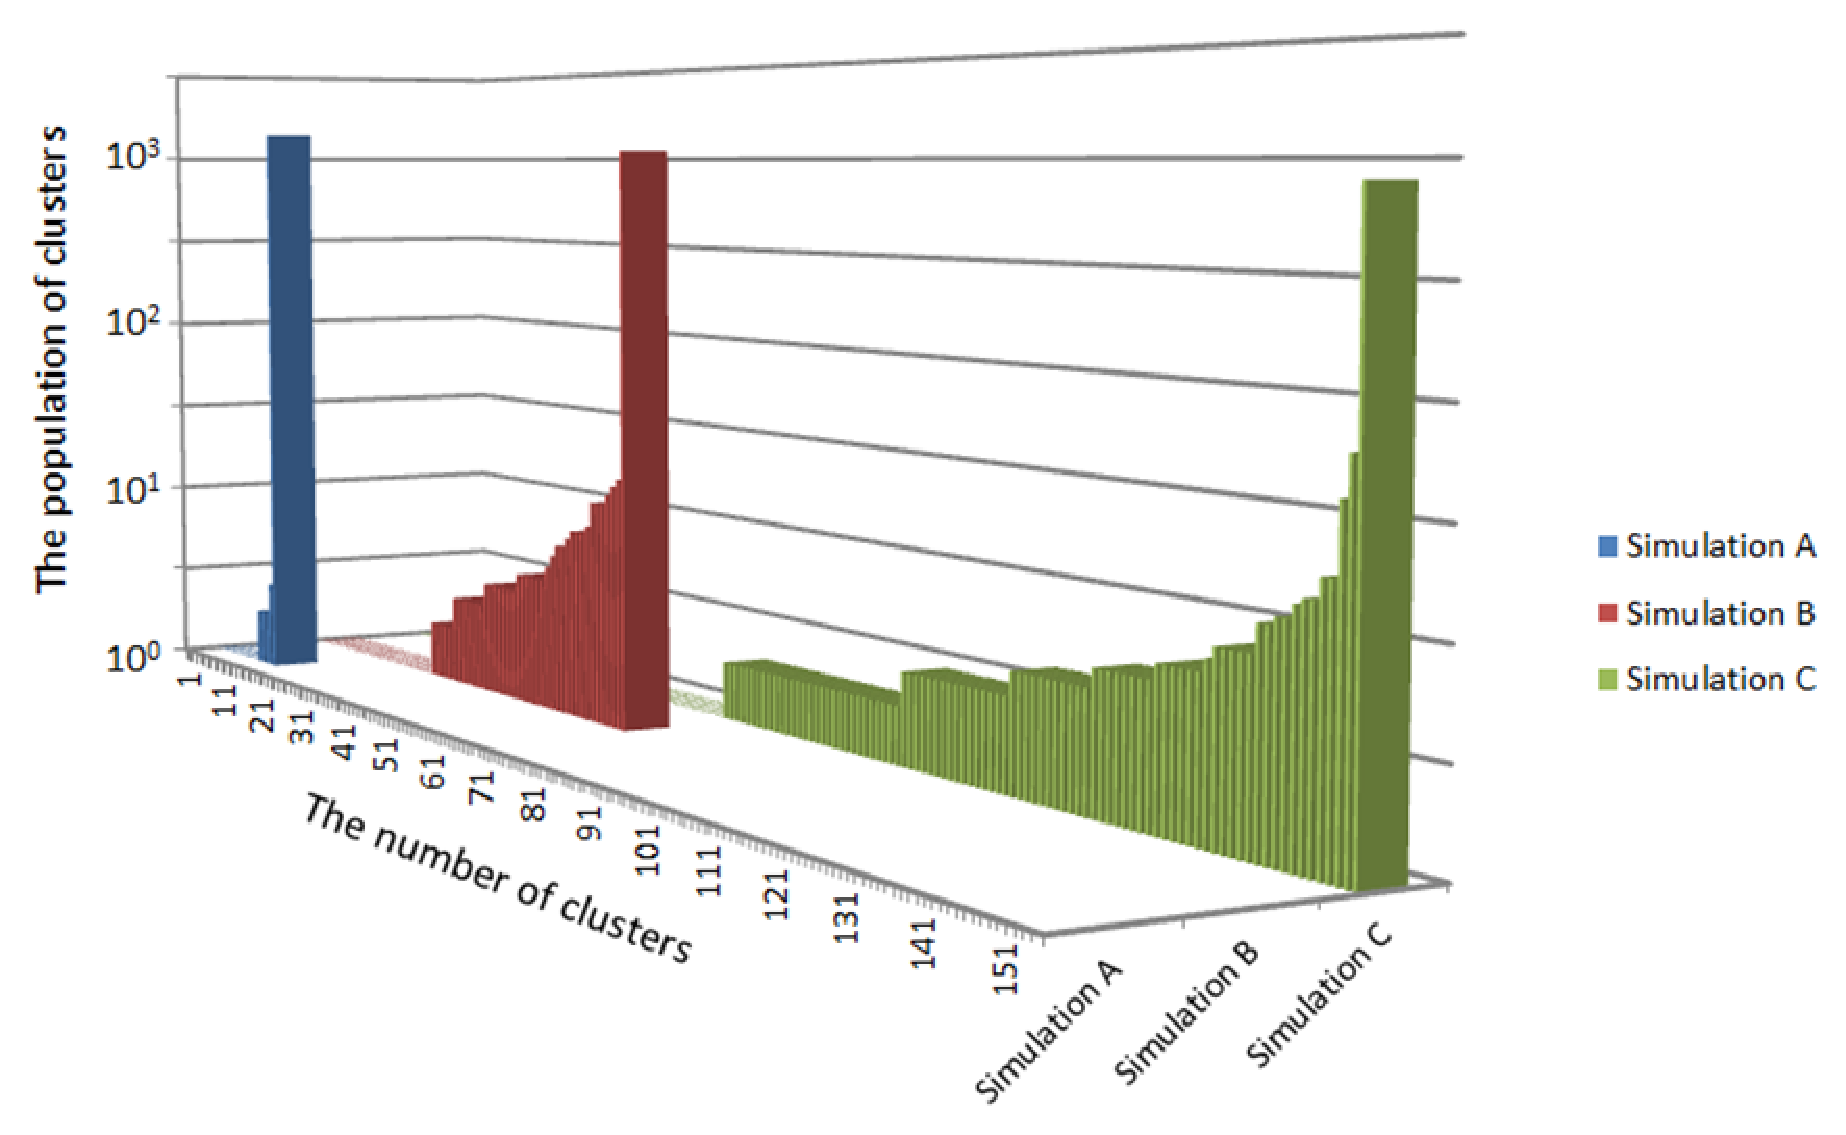
\epsfig{file=figs/cluster_population.eps, width=5.0in}
\caption{The number of created clusters and the population of clusters}
\label{fig:population}
\end{figure}
%
\begin{table}
\centering
\caption{Simulation setup with various parameters setup}
	\begin{tabular}{c|c|c|c|c}
	\hline
	\ & \textit{D$_{max}$} & \textit{S$_{min}$} & $\alpha$$_{distance}$ &
$\alpha$$_{size}$ \\
	\hline
	Simulation A & 200ms & 200 & 0.3 & 0.7 \\
	Simulation B & 100ms & 100 & 0.5 & 0.5 \\
	Simulation C & 50ms & 50 & 0.7 & 0.3 \\
	\hline
	\end{tabular}
\label{table:simulation_setup}
\end{table}
%
\begin{figure}
\centering
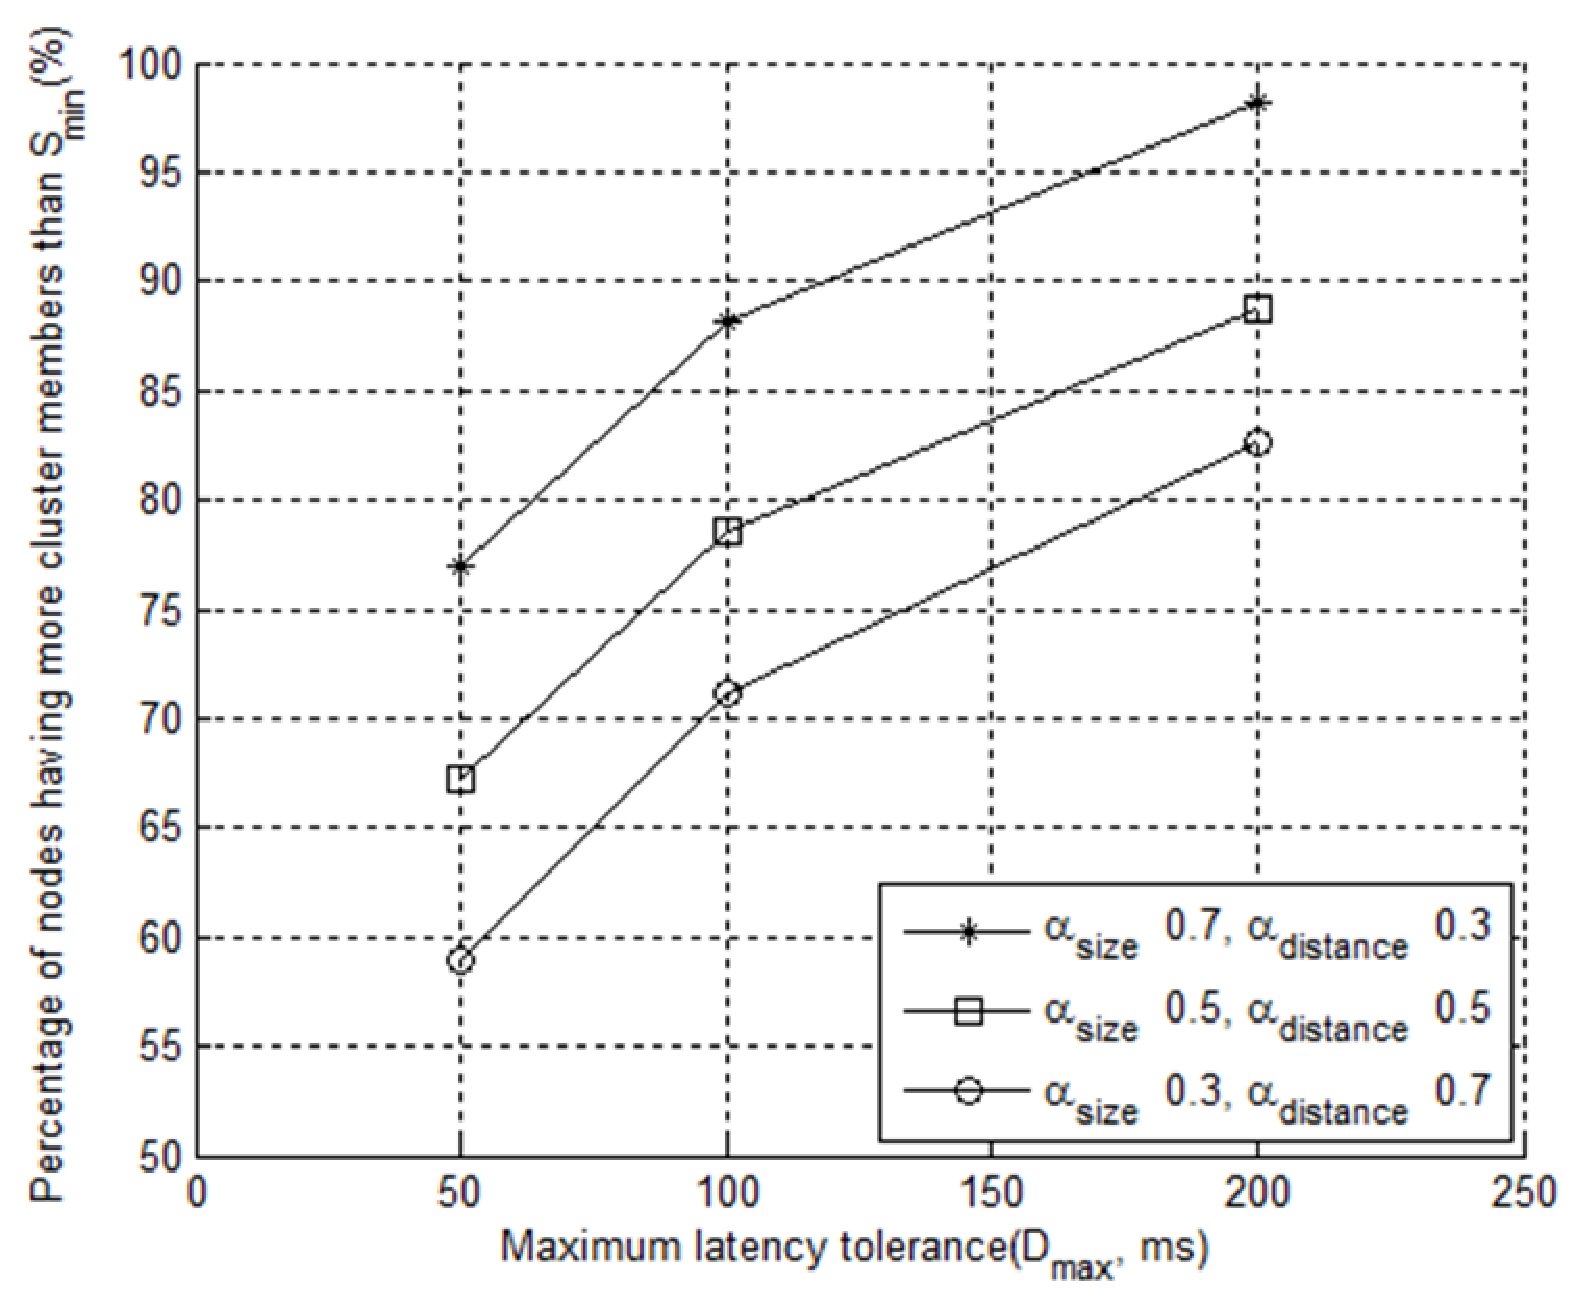
\epsfig{file=figs/percentage_s50.eps, width=4.0in}
\caption{Percentage of nodes having more cluster member than \textit{S$_{min}$} = 50}
\label{fig:population50}
\end{figure}
%
\begin{figure}
\centering
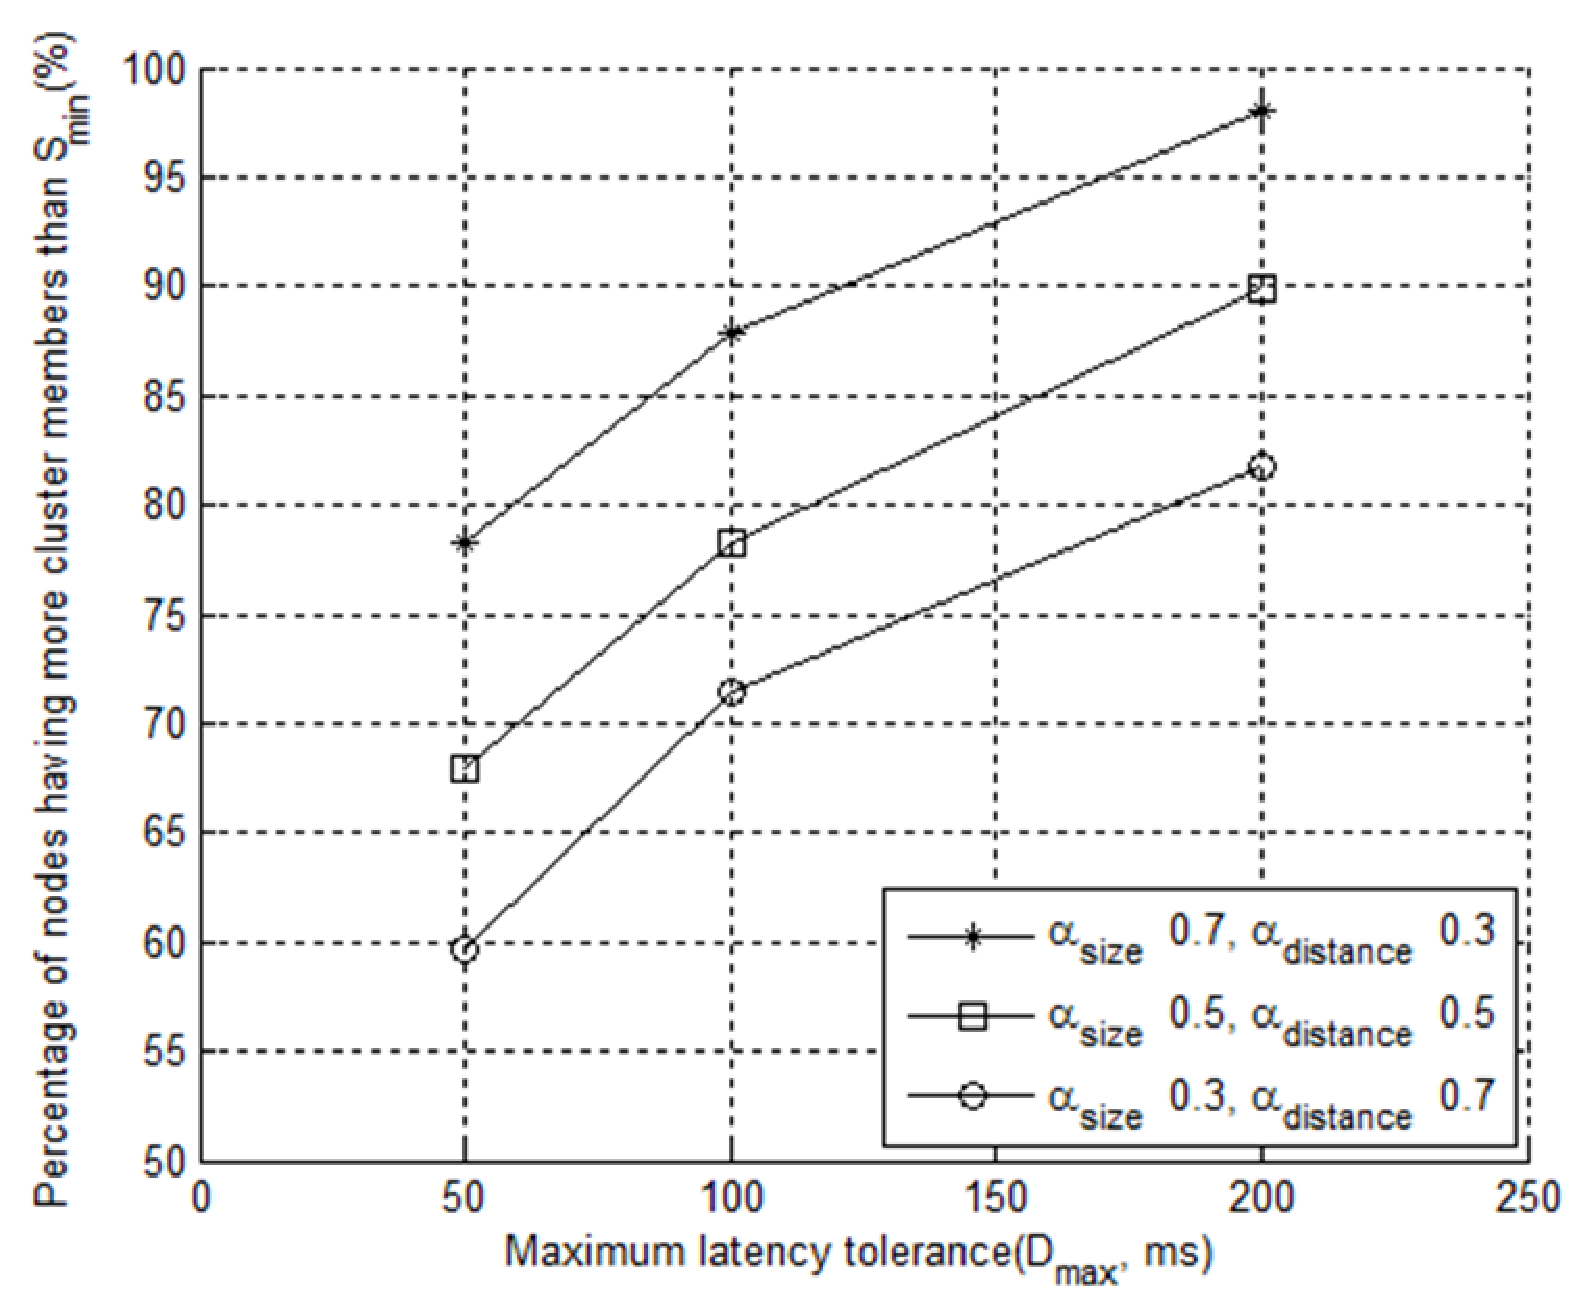
\epsfig{file=figs/percentage_s100.eps, width=4.0in}
\caption{Percentage of nodes having more cluster member than
\textit{S$_{min}$} = 100}
\label{fig:population100}
\end{figure}
%
\begin{figure}
\centering
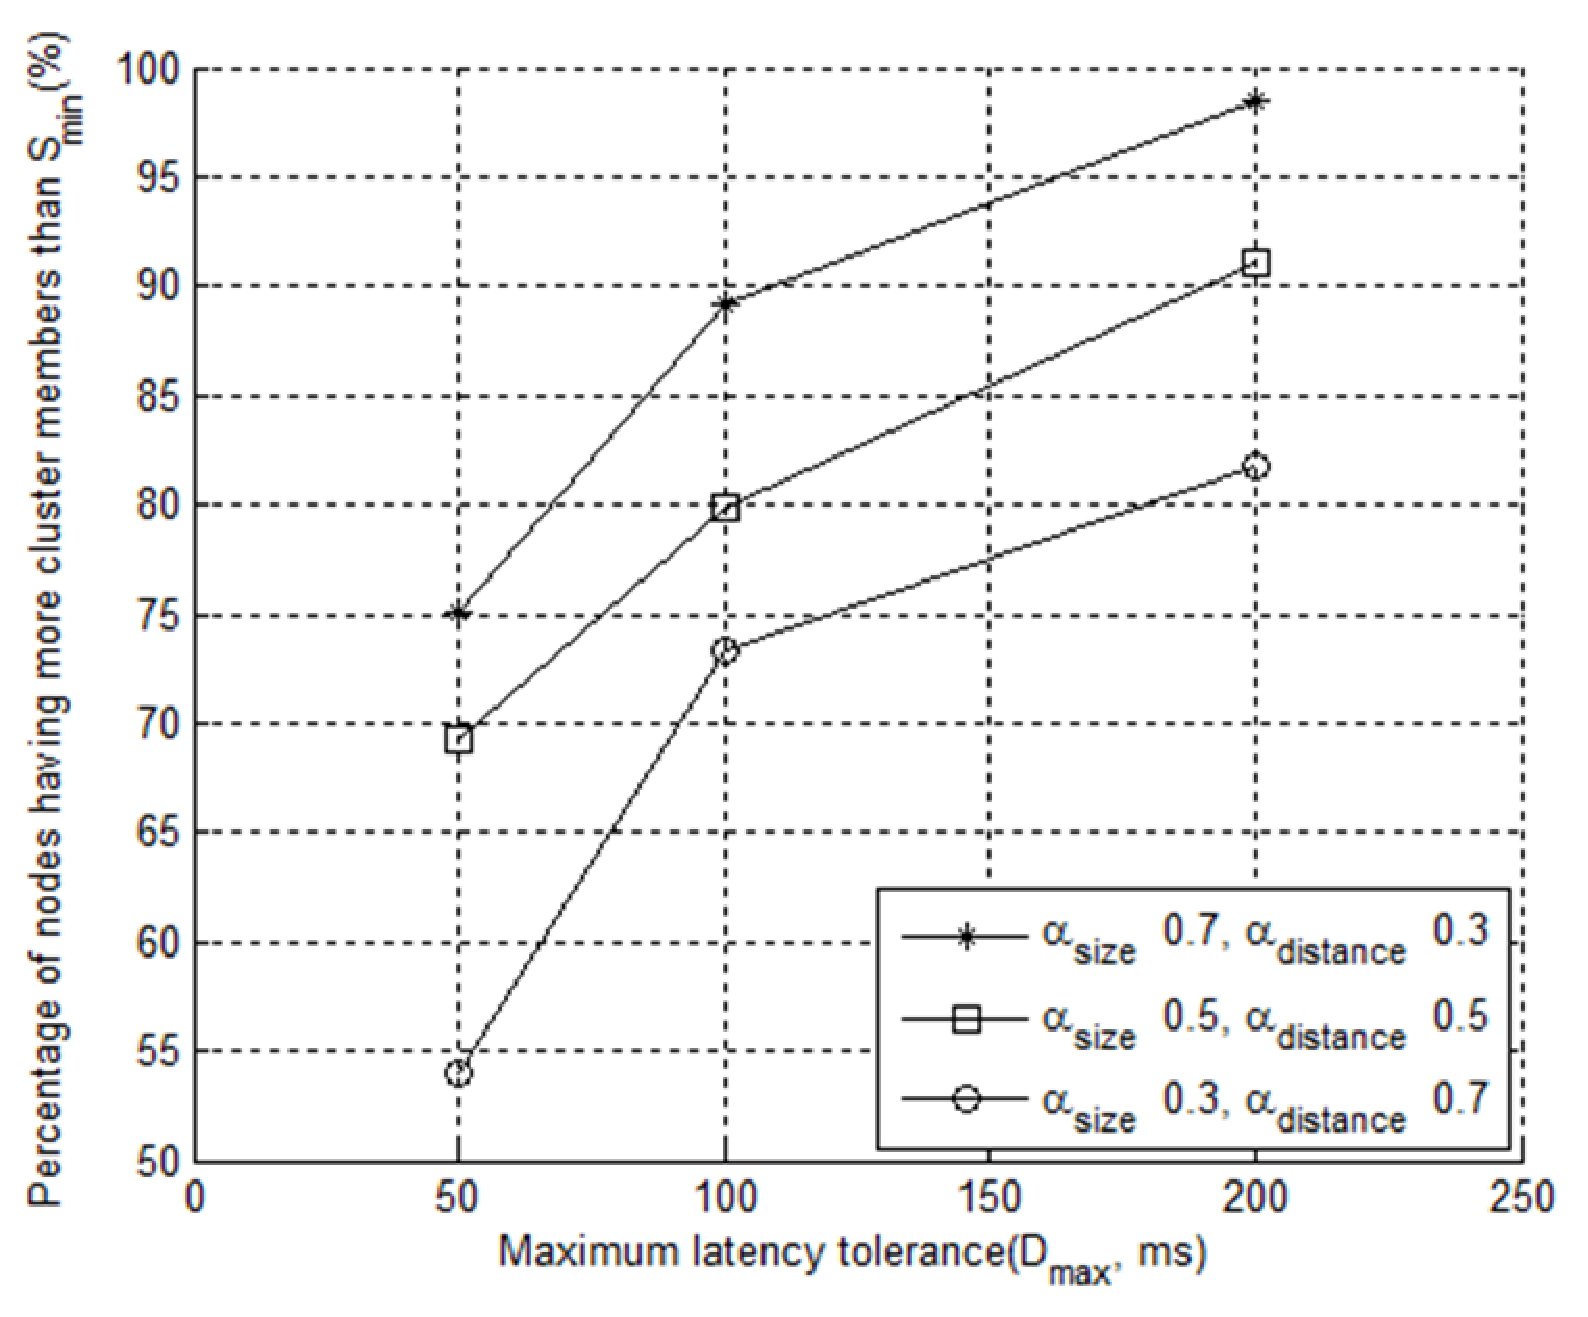
\epsfig{file=figs/percentage_s200.eps, width=4.0in}
\caption{Percentage of nodes having more cluster member than
\textit{S$_{min}$} = 200}
\label{fig:population200}
\end{figure}

\subsection{The number of cluster members}
\label{solare:clustermember}
In addition to intra-cluster latencies, I measure the cluster size which
takes the other part of total utility function.
%
To measure the cluster size, I took snapshots of the number of created
clusters and cluster members for each node when all nodes join a
cluster.
%
Due to the limitation of space, the results from only three simulations
of all the simulations I performed are represented in
Figure~\ref{fig:population} depicting the number of created clusters and
the population of clusters.
%
Table~\ref{table:simulation_setup} summarizes the parameters setup for
the simulation.
%
Firstly, in simulation A, I observe that only 16 clusters are created
and 98.5\% of nodes are included in only one cluster.
%
In fact, for this simulation set, \textit{D$_{max}$} and
$\alpha$$_{size}$ are set to 200ms and 0.7 which are most likely to
organize the largest cluster of all the simulations.
%
However, as \textit{D$_{max}$} and $\alpha$$_{size}$ decrease, the number
of created clusters increases and the population is also distributed
throughout the created clusters.
%
Particularly, for the case of simulation C in which nodes require
relatively small cluster size but much closer cluster members, 155
clusters are created and nodes join clusters more evenly than simulation
A or B.
%
Furthermore, each result from three simulations show one big cluster
including at least 58\% of nodes which is caused by the type of utility
function for cluster size I used.
%
From Chapter~\ref{solare:utility}, recall the baseline of utility
function for cluster size in such that nodes prefer larger cluster size
without an upper limit.
%
If I consider another type of utility function which defines upper limit
of cluster size, one major cluster may disappear and the population of
cluster should become more even.\\
%
To summarize the evaluation of quantitative performance, as shown in
Figure~\ref{fig:population50},~\ref{fig:population100},
and~\ref{fig:population200}, I consider the percentage of nodes which have more cluster
members than \textit{S$_{min}$}.
%
Figure~\ref{fig:population50} shows that as \textit{D$_{max}$} and
$\alpha$$_{size}$} become larger, more nodes can obtain same or
more cluster members than \textit{S$_{min}$} 
%
Although, indeed, only 54\% of nodes have more cluster members than
\textit{S$_{min}$} with 50ms of \textit{D$_{max}$} and 0.3 of
$\alpha$$_{size}$, in the case with 200ms of \textit{D$_{max}$} and 0.7
of $\alpha$$_{size}$, almost 98\% of nodes satisfy the minimum
preference for cluster size, \textit{S$_{min}$}.
%
Regardless of setting of \textit{S$_{min}$}, the same trend is observed
in Figure~\ref{fig:population100} and~\ref{fig:population200} where
\textit{S$_{min}$} is set to 100ms and 200ms with more than 97\% and
98\% of nodes satisfied with \textit{S$_{min}$}.
%
Thus, I can confirm the correctness of this clustering system with the
result of the number of cluster members.
%

\subsection{Adaptability to dynamic network conditions}
\label{solare:adaptability}
Finally, I discuss the adaptability of SOLARE.
%
Network status can be changed dynamically due to the node joining,
leaving, and the change of network latencies.
%
Therefore, nodes should adapt to dynamic network status for the ability
to self-manage the cluster system.
%
After a node joins the cluster, it periodically updates the utility for
its cluster, so if utility is dropped below the threshold, a node
repeats the cluster joining procedure to migrate into another high
utility-valued cluster.
%
To evaluate the adaptability of this system, I observe the percentage of
the number of nodes which need the cluster migration and average utility
value over the entire network.
%
Instead of directly modifying network latency at the simulation
environment, I assume that new joining in global network can cause the
change of the position of nodes in the network coordinate space.
%
Figure~\ref{fig:rejoin} shows the percentage of the number of nodes
which need to migrate from current cluster into another cluster due to
the negative utility value.
%
Because 1740 nodes sequentially join in global network with 500
milliseconds of interval in the simulation scenarios as described in
Table~\ref{table:simulation_setup}, all nodes complete joining the
global network around 15 minutes after starting the simulation.
%
In the case of simulation A where \textit{D$_{max}$} and
\textit{S$_{min}$} are set to 50ms and 50, respectively, cluster
migrations happen most frequently.
%
In fact, because parameters for simulation C imply the smallest cluster,
it is most likely that cluster migrations occur by slight change of the
coordinate.
%
However, after all nodes join the global network and step into correct
position, the occurrence of migrations decreases and the percentage of
nodes which migrate to another cluster is dropped below 5\% after 30
minutes from starting the simulation.\\
%
\begin{figure}
\centering
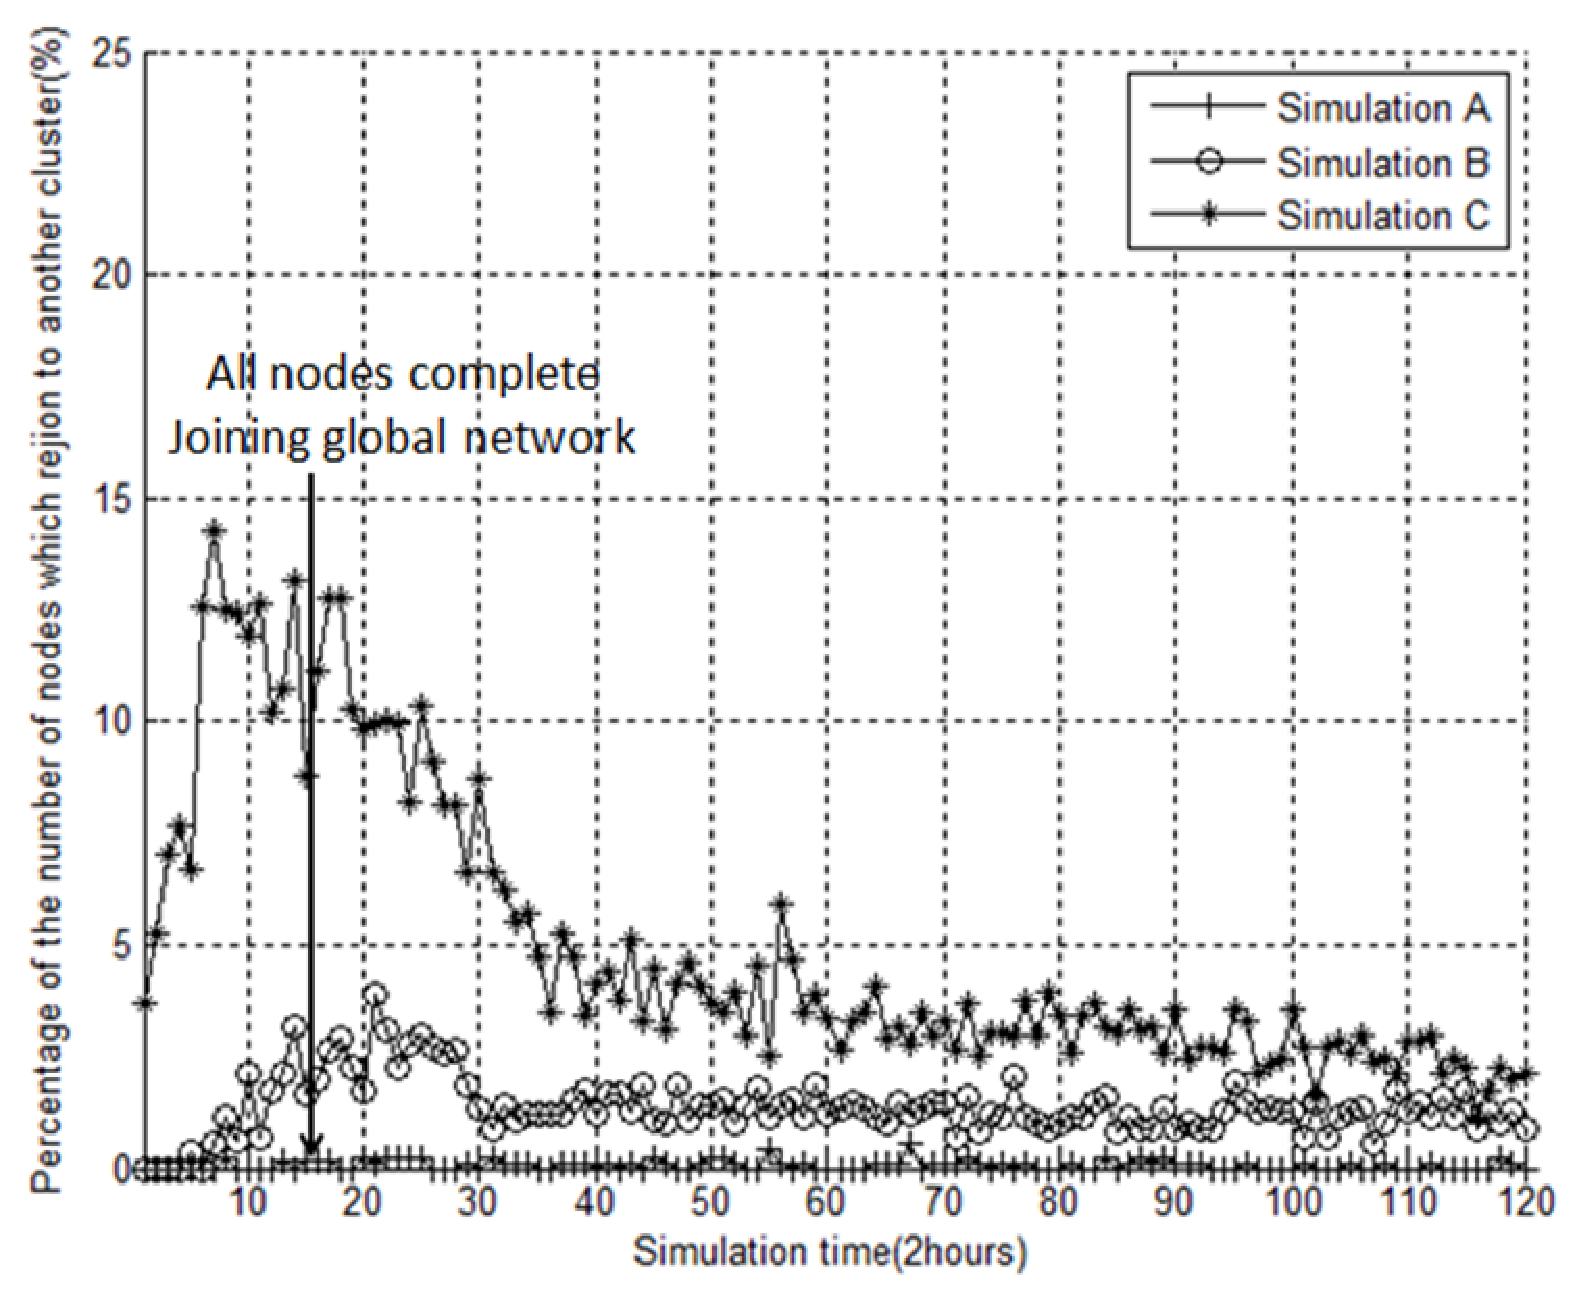
\epsfig{file=figs/rejoin.eps, width=4.0in}
\caption{Percentage of the number of rejoining nodes}
\label{fig:rejoin}
\end{figure}
%
\begin{figure}
\centering
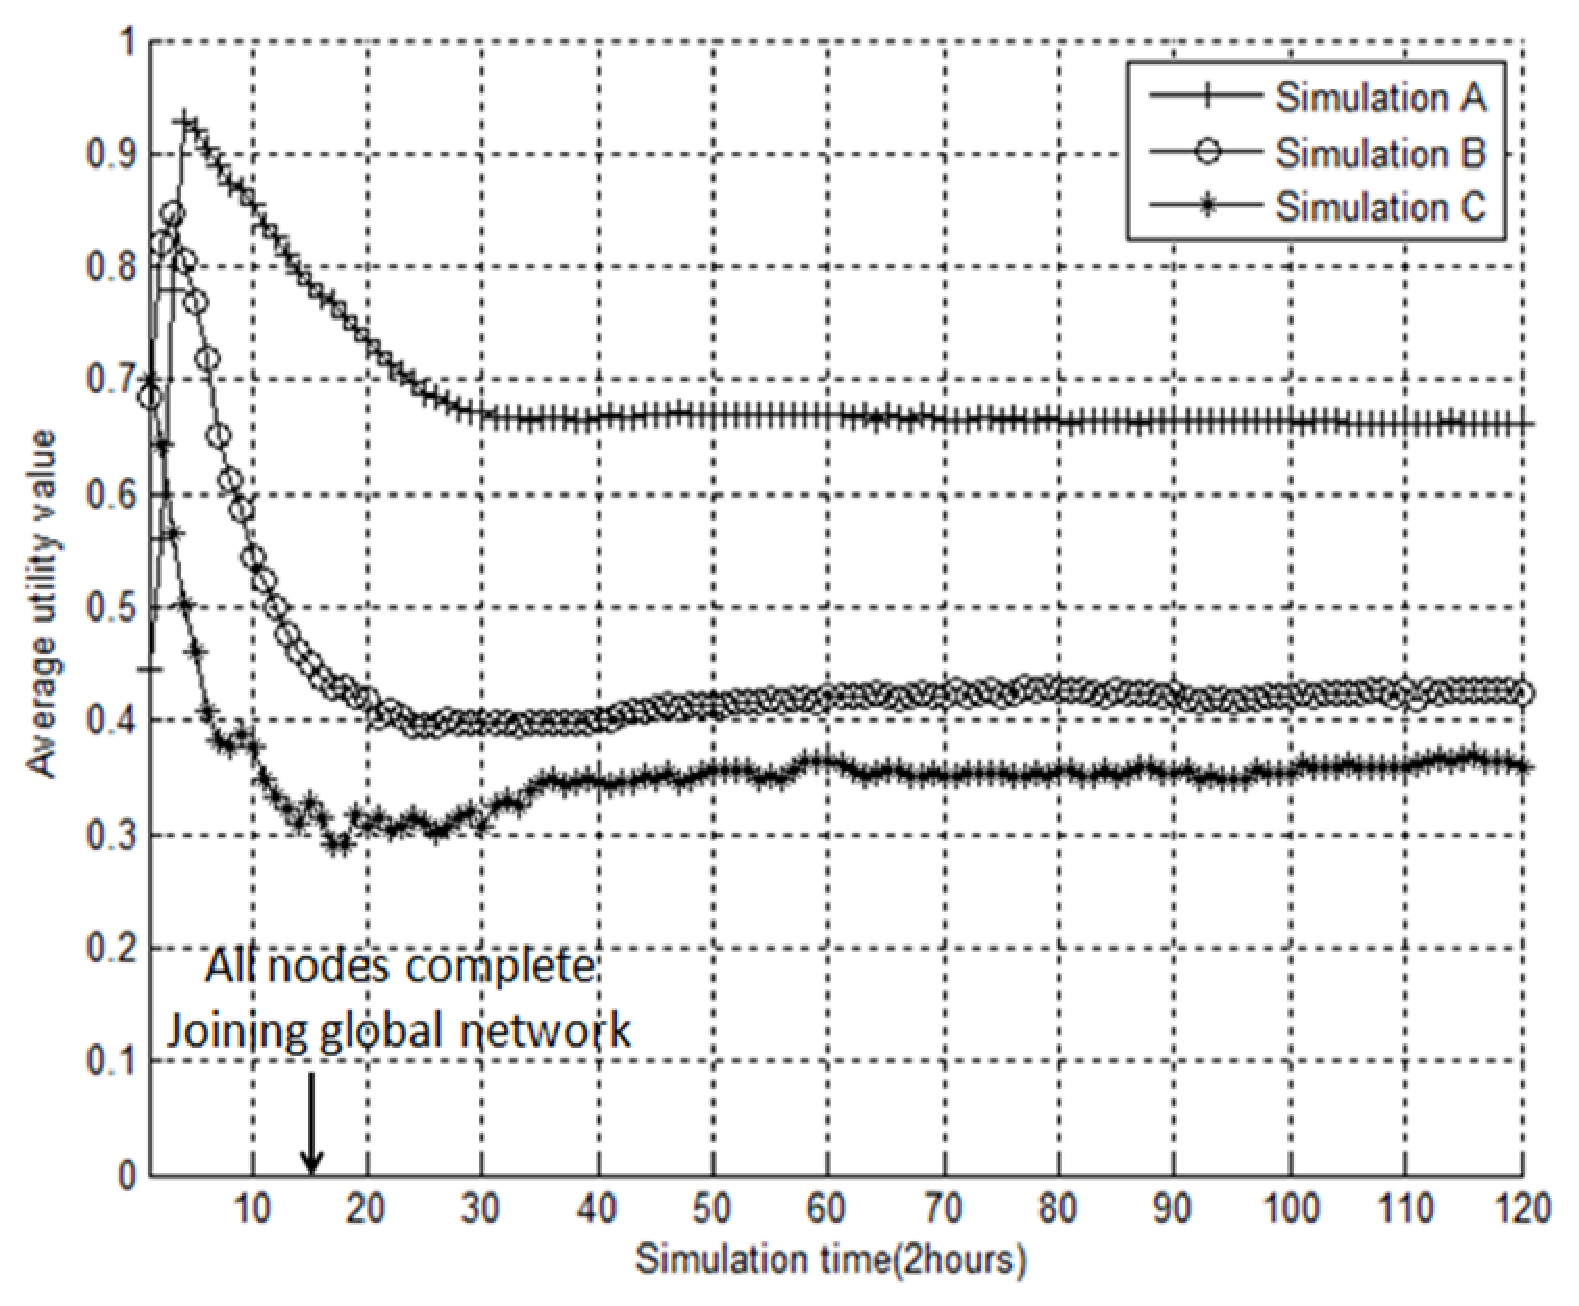
\epsfig{file=figs/average_utility.eps, width=4.0in}
\caption{Average utility value}
\label{fig:avgutility}
\end{figure}
%
Such a pattern of the occurrence of migrations is observed in the case
of simulation B with 100ms of \textit{D$_{max}$} and 100 of
\textit{S${min}$}, but the percentage of nodes which migrate into
another cluster is less than simulation C because of the parameters set
which means bigger cluster than the case of simulation C.
%
Especially, in Simulation A where the biggest cluster is set, nodes
barely migrate, because the change of the coordinate of nodes occurs
within a cluster.
%
Also, I can observe from Figure~\ref{fig:avgutility} that after the
percentage of nodes which migrate is saturated or dropped drastically,
the average utility value over the entire network is also saturated
which means that the majority of nodes place at correct position and
stay in current cluster.
%
Note that the difference of the utility value saturated can be inferred
from Figure~\ref{fig:population}.
%
Because most of nodes with simulation A, about 98.5\%, are in the same
cluster, it is easy to gain higher utility value for cluster size than
other cases.
%
On the other hand, in the case of simulation C, nodes are distributed
among many clusters, and only 59\% of nodes have more cluster members
than \textit{S$_{min}$}.
%
Consequently, it results in the lowest utility value for cluster size
and total average utility value.
%
%\section{Possible Integration with Mobile Offloading Framework}
%\label{solare:integration}

\section{Summary}
\label{solare:summary}
In this Chapter, I introduced SOLARE, a peer-to-peer, utility based
self-organizing clustering system which is able to collaborate with
remote computation offloading to achieve the additional offloading
performance improvement.
%
Since the main goal of SOLARE is to organize a proximity-aware
clustering topology, it is possible to provide mobile offloading
framework with more resilient resource discovery service by supplying a
list of remote resources which have similar network performance. 
%
In SOLARE, all participants compute themselves the utility for existing clusters
and join highest utility valued cluster.
%
On the other hand, if there is no cluster whose utility is greater than
the user-defined threshold, nodes create a new cluster declaring their
own coordinate as the virtual center of cluster.
%
To establish utility functions, I select the distance to cluster and the
size of cluster as utility properties.
%
Furthermore, the clustering system provides the adaptability for dynamic
network status while each node monitors the cluster that it is currently
joining.
%
After describing the self-organizing and managing clustering procedure,
I evaluated its performance in terms of latencies of intra-cluster and
the number of cluster members.
%
Based on the evaluation, I confirmed that setting of parameters, which
form utility functions, can control the properties of clusters such as
latencies of intra-cluster and the population of clusters.
%
Additionally, by measuring the percentage of the number of nodes which
need to migrate into another cluster and average utility value, I
presented the adaptability of the system.
%
